 

\documentclass[journal]{IEEEtran}
%
 

\usepackage{cite}
\usepackage{multicol,lipsum}
\usepackage{amsmath,amssymb,amsfonts}
\usepackage{algorithmic}
\usepackage{graphicx}
\usepackage{textcomp}
\usepackage{xcolor}
\usepackage{booktabs}
%\usepackage[colorlinks,linkcolor=blue]{hyperref}
 \usepackage{hyperref}
\usepackage{enumerate}
%\usepackage{algorithm2e}
\usepackage{algorithm}
\usepackage{multirow}
\usepackage{standalone}
\usepackage{tikz}
\usetikzlibrary{positioning}
\usetikzlibrary{decorations.markings}


  \usepackage{enumerate}
 %s \usepackage{caption}
\usepackage{subcaption}
 \usepackage{setspace}
\usepackage{verbatim}
   \usepackage{tabularx}
 \usepackage{makecell}
    \renewcommand{\algorithmicrequire}{\textbf{Input:}}
\renewcommand{\algorithmicensure}{\textbf{Output:}}
 \usepackage{hyperref}
 
 

% *** GRAPHICS RELATED PACKAGES ***
%
\ifCLASSINFOpdf
  % \usepackage[pdftex]{graphicx}
  % declare the path(s) where your graphic files are
  % \graphicspath{{../pdf/}{../jpeg/}}
  % and their extensions so you won't have to specify these with
  % every instance of \includegraphics
  % \DeclareGraphicsExtensions{.pdf,.jpeg,.png}
\else
  % or other class option (dvipsone, dvipdf, if not using dvips). graphicx
  % will default to the driver specified in the system graphics.cfg if no
  % driver is specified.
  % \usepackage[dvips]{graphicx}
  % declare the path(s) where your graphic files are
  % \graphicspath{{../eps/}}
  % and their extensions so you won't have to specify these with
  % every instance of \includegraphics
  % \DeclareGraphicsExtensions{-eps-converted-to.pdf}
\fi
% graphicx was written by David Carlisle and Sebastian Rahtz. It is
% required if you want graphics, photos, etc. graphicx.sty is already
% installed on most LaTeX systems. The latest version and documentation
% can be obtained at: 
% http://www.ctan.org/pkg/graphicx
% Another good source of documentation is "Using Imported Graphics in
% LaTeX2e" by Keith Reckdahl which can be found at:
% http://www.ctan.org/pkg/epslatex
% 




 


% correct bad hyphenation here
 

\begin{document}
%
% paper title
% Titles are generally capitalized except for words such as a, an, and, as,
% at, but, by, for, in, nor, of, on, or, the, to and up, which are usually
% not capitalized unless they are the first or last word of the title.
% Linebreaks \\ can be used within to get better formatting as desired.
% Do not put math or special symbols in the title.
\title{A Design of Low-Projection SCMA Codebooks  for Ultra-Low Decoding Complexity in Downlink IoT Networks }
%
%
% author names and IEEE memberships
% note positions of commas and nonbreaking spaces ( ~ ) LaTeX will not break
% a structure at a ~ so this keeps an author's name from being broken across
% two lines.
% use \thanks{} to gain access to the first footnote area
% a separate \thanks must be used for each paragraph as LaTeX2e's \thanks
% was not built to handle multiple paragraphs
%

\author{Qu Luo,   ~\IEEEmembership{Graduate Student Member,~IEEE,}
      Zilong Liu, ~\IEEEmembership{Senior Member,~IEEE,}
       Gaojie Chen, ~\IEEEmembership{Senior Member,~IEEE,} 
       Pei Xiao, ~\IEEEmembership{Senior Member,~IEEE,}
          Yi Ma, ~\IEEEmembership{Senior Member,~IEEE }
          and  Amine  Maaref,~\IEEEmembership{Senior Member,~IEEE.}  
\thanks{ Qu  Luo, Gaojie Chen,  Pei  Xiao  and Yi Ma are  with  5G \& 6G  Innovation Centre, Institute for Communication Systems (ICS), University of Surrey, UK, email:\{q.u.luo,  gaojie.chen, p.xiao, m.yi\}@surrey.ac.uk.}% <-this % stops a space
\thanks{ Zilong   Liu   is   with   the   School   of   Computer   Science   and   Electronic   Engineering,   University   of   Essex,   UK,    email:   zilong.liu@essex.ac.uk.}% <-this % stops a space
\thanks{ Amine  Maaref  is   with   the  Canada Research Center, Huawei Technologies Company Ltd., Ottawa, Canada,  email:  amine.maaref@huawei.com.}% <-this % stops a space
 }
 

 
\markboth{ } 
{Qu \MakeLowercase{\textit{et al.}}: A  Design of Low-Projection  SC Codebooks   that Enables Low Decoding Complexity for Downlink SCMA}%
% The only time the second header will appear is for the odd numbered pages
% after the title page when using the twoside option.
% 
 



% make the title area
\maketitle

% As a general rule, do not put math, special symbols or citations
% in the abstract or keywords.
\begin{abstract} This paper conceives a novel sparse code multiple access (SCMA) codebook design which is motivated by the strong need for providing ultra-low decoding complexity and good error performance in downlink Internet-of-things (IoT) networks, in which a massive number of low-end and low-cost IoT communication devices are served.    By focusing on the typical Rician fading channels, we analyze the pair-wise probability of superimposed SCMA codewords and then deduce the  design metrics for multi-dimensional constellation construction and  sparse codebook optimization.  For significant reduction of  the decoding complexity, we advocate the key idea of projecting the multi-dimensional constellation elements to a few overlapped complex numbers in each dimension, called low projection (LP). An emerging modulation scheme, called golden angle modulation (GAM), is considered for multi-stage LP optimization, where the resultant multi-dimensional constellation is called LP-GAM.   Our analysis and simulation results show the superiority of the proposed LP codebooks (LPCBs) including one-shot decoding convergence and excellent  error rate performance. %With the proposed LBCPs, it is shown that only $3\%$ decoding complexity reduction by at least $97\%$ compared to that of the conventional codebooks,  whilst owning  large minimum Euclidean distance.  Some examples of the proposed  LPCBs are available at  \url{https://github.com/ethanlq/SCMA-codebook}. 
In particular,  the proposed LPCBs lead to decoding complexity reduction by at least $97\%$ compared to that of the conventional codebooks,  whilst owning  large minimum Euclidean distance.  Some examples of the proposed  LPCBs are available at  \url{https://github.com/ethanlq/SCMA-codebook}. 
 
% for massive access,  for LP, which can offer large mutual information and low  peak-to-average power ratio (PAPR). superiority   Numerical and simulation results show that both  significant  complexity reduction  and performance improvement can be achieved for the proposed LP codebooks (LPCBs). 

\end{abstract}

% Note that keywords are not normally used for peerreview papers.
\begin{IEEEkeywords}
Sparse code multiple access (SCMA),  golden angle modulation (GAM), codebook design,  Internet-of-things (IoT),  low complexity  detection, Rician channels.
\end{IEEEkeywords}






% For peer review papers, you can put extra information on the cover
% page as needed:
% \ifCLASSOPTIONpeerreview
% \begin{center} \bfseries EDICS Category: 3-BBND \end{center}
% \fi
%
% For peerreview papers, this IEEEtran command inserts a page break and
% creates the second title. It will be ignored for other modes.
\IEEEpeerreviewmaketitle



\section{Introduction}
% The very first letter is a 2 line initial drop letter followed
 
  
%  %Satellite communication networks as an enhanced and complementary part of the terrestrial
% communication infrastructure is expected to play a significant role in future Internet of Things (IoT)
% communication networks
  \IEEEPARstart{T}{he}     Internet-of-things (IoT) represents a revolutionary paradigm shift from the legacy human-centric networks (e.g., in 3G and 4G) to massive machine-type communications, where the latter is a major use case in the 5G-and-beyond mobile networks  \cite{FuqahaCommun}.
  Under this big picture, however, 
it is challenging to support the concurrent  communications of  massive IoT devices.  Due to the limited time-frequency resources, traditional  orthogonal multiple access (OMA) may be infeasible.   A disruptive technique for addressing such a challenge  is called non-orthogonal multiple access (NOMA) which permits several times of IoT devices larger than that in OMA systems communicating simultaneously \cite{SparseYu}. 
 
  
  
 
 
 
%\IEEEPARstart{T}{he} emerging Internet of Things (IoT) application scenarios, such as smart grid, precision agriculture,  and regions lacking infrastructure  (e.g., oceans, deserts, remote mountainous areas) have lead to  an urgent need to provide ubiquitous connective with satellite-based  (S-IoT) \cite{WangJoint}. The S-IoT has recently been demonstrated as an efficient solution to enable   massive  connectivity and ubiquitous   coverage  in a cost-effective manner for massive machine type communications (mMTC) in the future Internet of Things \cite{SatelliteSanctis}. 


 %With the explosive growth of various MTDs, while considering the practical satellite payload limitations, how to accommodate the massive and concurrent connection requests is becoming a foreseeable challenge in the realization of satellite-based IoT.

%  \IEEEPARstart{S}{atellite}-based Internet of Things (S-IoT) has recently been demonstrated as an efficient solution to enable   massive  connectivity and ubiquitous   coverage  in a cost-effective manner for massive machine type communications (mMTC) in the future Internet of Things \cite{SatelliteSanctis}.  
% Particularly, more and more IoT application scenarios, such as smart grid \cite{ghasempour2019internet}, precision agriculture,  and regions lacking infrastructure  (e.g., oceans, deserts, remote mountainous areas) have emerged with .
 
 
 %intelligent transportation systems, precision agriculture, forest fire prevention infrared monitoring, sea or high altitude video surveillance, mining production and storage, etc
 
%networks are expected to be widely deployed and extended using integrated/hybrid architectures on multiple geostationary orbit (GEO) satellites, non-geostationary orbit (NGSO) satellites (i.e., medium/low earth orbit (M/LEO) satellites) and terrestrial layers, along with emerging ke
 
 
% However, these areas tend to be large and terminal equipment is sparsely deployed.  Meanwhile, these areas need to
% support tens or even hundreds of kilometers of wireless communication technology to achieve wide-area networking and
% transmission, which cannot be met by traditional IoT technologies
 

 
%Recently, low earth orbit (LEO) satellite networks have
%developed rapidly and are considered to be an important component of next-generation mobile communication technologies. 

 % The key concept of NOMA is to enable multiple users, whose number is larger than that of their occupied resource nodes,  to communicate simultaneously  in   non-orthogonal manners.
% Consequently, the innovation concept of non-orthogonal multiple access (NOMA) has been proposed to achieve large-scale connectivity and high spectral efficiency \cite{islam2016power,cai2017modulation,7973146Survey} for mMTC networks. The basic concept of NOMA is to allocate the time/frequency resources to multiple users in non-orthogonal manners.  

Existing NOMA techniques can be mainly categorized into two classes: power-domain NOMA \cite{islam2016power}  and code-domain NOMA (CD-NOMA)  \cite{liu2021sparse}. The former works by superimposing multiple users with distinctive  power levels over the  identical time-frequency resources, whereas the latter carries out multiplexing  by employing different  codebooks/sequences with certain intrinsic structural properties. 
This paper focuses on  the sparse code multiple access (SCMA) \cite{taherzadeh2014scma, hoshyar2008novel }, which is a  representative CD-NOMA scheme with sparse codebooks. In SCMA, every user's  instantaneous input message bits  are directly mapped to a multi-dimensional sparse codeword drawn   from a pre-designed codebook \cite{luo2021error}.  
 SCMA is attractive as judiciously designed codebooks lead to constellation gain (due to signal space diversity), whilst their sparsity can be leveraged to enable near-optimum  message passing (MPA) decoding \cite{hoshyar2008novel}.
 
  Many studies have been carried out  to reap the benefits of SCMA for the enabling of massive connectivity in  IoT networks  \cite{AchievingZeng,SparseMoon,JointMiuccio,AnalyzingLai,ZhangComplexity,WangIterative}.  Recently, SCMA has also been applied in satellite IoT networks with novel  random access design \cite{ZhangUser,li2019asynchronous} and new receiver schemes  \cite{ZhangComplexity,WangIterative}. To realize these SCMA based IoT systems, nevertheless, a fundamental question is: \textit{how to design new sparse codebooks to enable highly efficient decoding in terms of complexity, energy/storage consumption, and convergence?} We will address this as detailed in the sequel. 
 
 %As the  IoT devices  are often low-end  sensors with stringent constraints in terms of battery life and computation/storage capabilities \cite{AnalyzingLai}, it is pivotal to design good sparse codebooks to permit excellent decoding error performance  and ultra-low decoding complexity.
 

% especially in an IoT system  where .
 
 
% A SCMA enhanced full-duplex  scheme  was proposed in  to achieve in IoT networks.  The random access (RA) of  SCMA for IoT networks has been studied in , which show  the   feasibility of the SCMA-based RA procedure  in supporting massive connectivity.  To reduce the signaling overhead and access delay in the RA process,   grant-free SCMA has been further   investigated \cite{PanGrant,AnalyzingLai}. In particular, the authors in \cite{AnalyzingLai} analyzed the error  performance of grant-free SCMA under codebook collision. The deployment of SCMA to satellite IoT networks has also been studied to some extent, where the satellite-to-terrestrial  channel is often characterized by  Rician fading channels \cite{5G_NR_s_iot,lutz1991land, vucetic1992channel}.   %In  \cite{gui2021scma}, the authors proposed an SCMA based secure communication scheme for  satellite-terrestrial network. 
%The  grant-free SCMA based    satellite IoT  network  has been   investigated  in \cite{li2019asynchronous}.  In \cite{ZhangComplexity}, a modified   approximate message passing detector that enable low complexity decoding  was proposed for SCMA-based  low earth orbit (LEO) satellite communications.  Very recently, the authors in \cite{WangIterative}   proposed  a  novel turbo iterative detection   detector in SCMA based satellite-terrestrial network  to eliminate the  multi-user interference and time-varying Doppler shifts.
 
 \subsection{Related works}



%The authors in \cite{NonPerez} studied  the application of various NOMA schemes in satellite communications, which shows that  NOMA schemes  are suitable for  providing massive connectivity in the downlink  satellite  communications.  Overall, the above works show  the  feasibility of the SCMA-based multiple access  in supporting massive connectivity for future S-IoT networks. However, none of the above work has touched the efficient sparse codebook design.

% In , the authors introduced a novel uplink grant-free asynchronous flipped SCMA   scheme for  future S-IoT  networks. 
%The PD-NOMA based  multiple access for satellite communications has been  investigated extensively in terms of   outage probability \cite{YueOutage,YanPerformance}, resource allocation \cite{JointZhao,MirboloukRelay}, random access \cite{TubianaLearning, MaNovel} and etc.   Considering the tiny power differences among different users in one satellite beam, the SCMA scheme may has stronger potential for  S-IoT networks.  

 
  
%The random access (RA) of  SCMA for IoT networks has been studied in \cite{SparseMoon,JointMiuccio}, which shows the   feasibility of the SCMA-based RA procedure   in supporting massive connectivity.  To reduce the signaling overhead and access delay in the RA process,   grant-free SCMA has been further investigated. Specifically,  \cite{li2019asynchronous} introduced a novel uplink grant-free asynchronous flipped SCMA   scheme for   future S-IoT communication networks. The error   performance of grant-free SCMA under codebook collision was analyzed   in \cite{AnalyzingLai}.


  In SCMA literature, to avoid the excessive design complexity, a widely adopted approach is to apply certain  user-specific operations (e.g., interleaving,    permutation, shuffling and phase rotations) to a common multidimensional constellation, called a   mother constellation (MC), for multiple sparse codebooks   \cite{nikopour2013sparse,taherzadeh2014scma}.   Following this approach, various types of SCMA codebooks have been developed in \cite{mheich2018design,cai2016multi,deka2020design,yu2015optimized,Zhang,li2020design,chen2020design}.  For excellent error performance, it is desirable to maximize the   minimum product distance (MPD) or minimum Euclidean distance (MED) of an MC \cite{boutros1996good}. In general, a large MED  leads to reliable detection in the Gaussian   channel, whereas a large MPD is preferred for robust transmissions in the Rayleigh fading channel \cite{WenDesigning}.
For example, the authors in \cite{cai2016multi} proposed a simple constellation rotation and interleaving  codebook design scheme  by using  an MC with enlarged MED.  
Golden angle modulation (GAM)  constellation was adopted in   \cite{mheich2018design}  to construct SCMA codebooks with low  peak-to-average power ratio (PAPR) properties.  
In \cite{yu2015optimized}, Star-QAM constellation was introduced to construct MC with large MED for downlink SCMA.   
In addition, a  uniquely decomposable constellation group   based codebook design approach was developed  in \cite{Zhang} by maximizing the MED at each resource node. With the aid of generic algorithm, in \cite{li2020design}, a  novel class of power-imbalanced SCMA codebooks  was developed in \cite{li2020design} by maximizing    the MED of the superimposed codewords whilst maintaining a large  MPD of the MC.   Recently, new downlink  quaternary sparse codebooks with large MED were obtained in \cite{huang2021downlink}  by a new iterative algorithm based on alternating maximization with exact penalty.     %A $4$-ary codebook with large MED in the SCMA system of $4$ resource nodes and $6$ users is obtained by solving  non-convex problem  with an alternating maximization approach. % Unfortunately, due to the overwhelming variables and complexity, it is very challenging, if not impossible, to obtain a higher rate codebook or a codebook of higher overloaded system.  
%  \footnote{For simplicity, we denote the SCMA system in which $J$ users communicate over $K$ resource nodes as ($K \times J$).}

%Many low-complexity receivers based on modified MPA have been proposed to reduce the computation cost of SCMA decoding \cite{LowYang,FastYang,ShuffledYang}.
It is worth mentioning that  the complexity  of MPA decoding can be significantly  reduced by  designing an MC  with low projection   (LP) numbers \cite{bayesteh2015low,bao2017bit}. This is achieved by allowing  certain overlapped constellation elements at the same dimension. The rationale is that, due to the multidimensional nature, any two MC vectors with certain overlapping dimension(s) may be well separated in other  dimension(s). Importantly, constellation overlapping at certain dimension (or more) leads to less computations in the message passing based inference.  By leveraging this advantage, the authors in \cite{bayesteh2015low}  proposed a modified LP-MPA decoder which  can utilise the  constellation structure to reduce    the  number of calculations of  belief messages  at each iteration.     Subsequently, the authors in   \cite{bao2017bit} presented an LP codebook design based on   the amplitude phase-shift keying   constellation in each dimension in uplink SCMA systems.  
To the best of our knowledge, a comparative study on sparse codebooks  with LP numbers in downlink channels is still missing.  This is challenging because one  needs to deal with the difficulties for joint optimization of the MC and user-specific codebook operators as well as the prohibitively high computational complexity in calculating the minimum Euclidean/product distance  of  the superimposed codewords. 
 
 
 
%  %In \cite{ZhangSparse}, the log-MPA is employed to avoid computing  exponential operations. The authors in \cite{LowYang,FastYang,ShuffledYang,ImprovedDai}  reduce the decoding complexity by modifying the message update equations to have fast convergence and less number of iterations. In addition, 
%  \cite{LowWei,bayesteh2015low} proposed low complexity detection techniques by taking advantage of a class of codebooks which have low number of projections.  
 
 \subsection{Motivations and contributions} 

This paper is driven by the key observation that a majority of IoT communication devices  are usually low-end and lost-cost wireless sensors which are very constrained in terms of resources such as energy, CPU, and memory/storage capacity\footnote{One may refer to  \cite{HahmOperating} for an excellent survey on low-end IoT devices as well as their major challenges posed to the operating system design.}.
%Because of this, it is desirable to design new SCMA decoding algorithm to have extremely low complexity and super-rapid convergence rate. 
In view of this and unlike many existing SCMA papers focusing on efficient receiver design, we aim for achieving extremely low decoding complexity and super-rapid convergence rate at the receiver from the codebook design perspective. In addition, in spite of numerous SCMA codebook designs for Gaussian channels or Rayleigh fading channels, they may not be optimal for other real-life  channels.   Typically, a practical wireless channel consists of a  small-scale fading caused by non-line of sight (NLoS) propagation and static line of sight (LoS) path, which can be modeled as Rician fading channels.  The Rician fading channels are widely present  in practical IoT networks, such as the  terrestrial IoT networks \cite{ZhangPerformance,YuCost},   satellite IoT  networks \cite{5G_NR_s_iot,lutz1991land, vucetic1992channel,li2019asynchronous,gui2021scma,ZhangComplexity,WangIterative}, and unmanned aerial vehicle (UAV)  networks \cite{ErnestNOMA,WangTrajectory}. 

The above observations     motivate  us to design   enhanced codebooks  that  can substantially  reduce the decoding complexity, while   achieving good error   performance for SCMA based downlink IoT networks under Rician  fading channels. The main contributions of this work are summarized as follows:

%This is in sharp contrast to the LP codebook design in \cite{bayesteh2015low} and  \cite{bao2017bit} for uplink SCMA channels where the decoding is carried out at an advanced base-station receiver.  Furthermore, the codebook design in downlink channels needs to deal with the difficulties for joint optimization of the MC and user-specific codebook operators as well as the prohibitively high computational complexity in calculating the MED  of  the superimposed codewords.






%the computation capability of IoT terminals such as sensors, are generally  extremely limited.  Although  the authors in  \cite{bao2017bit} present a class of SCMA codebook that enable low complexity of detection, it only covers the MC design for uplink Rayleigh fading channel.  In downlink channels, the codebook design is a more challenging problem due to the difficulty of  joint design the MC and   users' constellation operators,  and the  overwhelming   Therefore, the design of SCMA codebooks that can reduce the computational complexity is even  more practical significant and beneficial in downlink S-IoT networks. 

 %inefficiently applied to the straightforward SAT-IoT networks

%It is also worth to mentioning that  the optimal SCMA codebook is  channel-dependent and the above  codebook design  mainly focus on the cellular communication networks by whether assuming AWGN or Rayleigh fading channels.  However, in general,  the satellite channels are more complex than cellular communication networks. As reported by 3rd Generation Partnership Project (3GPP) in TR 38.811 \cite{5G_NR_s_iot},  the user in open, suburban and rural scenarios mainly experience a line-of-sight (LOS) propagation, and the LoS probability for  urban and dense urban area varies from $28.2\%$ to $99.2\%$, which   depends on the UE environment and elevation angle.  In fact, the Rician fading channel can sufficiently describes the characteristic of satellite-to-terrestrial link with an LoS path, thus it is widely employed in the existing literature \cite{lutz1991land, vucetic1992channel }. Unfortunately, the design of SCMA codebook for S-IoT networks characterized by a general Rician fading channel  is still missing, and  the corresponding design KPI is also unknown.
 

%However, it is also of interest to investigate  the codebook design in a more general Ricain channel model. Not only this generalize the previous derived design criteria, %since both AWGN and Rayleigh fading channels can be considered to be limiting cases of Rician channel,  
%but Ricain fading is also known to be a better model for wireless environment with a line of sight (LOS) path \cite{stuber1996principles}. 
%The primary objective of this paper is to design enhanced SCMA codebooks that can  reduce the decoding complexity, while at the same time, achieve good error rate performance in downlink Rician fading channels.
% In this paper,By analysing
% the pair-wise probability (PEP) in downlink Rician fading channel,
% the design criteria for MC construction
% and sparse codebook optimization are first established.   Then, a simple multi-stage approach is proposed to construct the sparse codebooks with low projected numbers.  


\begin{itemize}
  \item 
  We analyze  the  system performance of SCMA in downlink Rician fading channels, and  derive the minimum distance of the  superimposed  codewords   by investigating  and minimizing the conditional  PEP. It is shown that our   derived minimum distance  generalizes  the previous design metrics, i.e., the MED and MPD, which are for the AWGN and Rayleigh fading channels, respectively.
 
  
  \item We propose a novel class of LP codebook (LPCB) to   enable  ultra-low   decoding complexity  and   excellent   error
performance.  Specifically, an efficient algorithm  is first proposed to  construct a novel  one-dimensional basic constellation with  proper LP numbers based on GAM  (LP-GAM)\footnote{GAM is an emerging  modulation that  leads to higher  mutual information and lower  PAPR performance over pulse-amplitude modulation   and square quadrature amplitude modulation (QAM) \cite{larsson2017golden}.}.  Afterwards, general multi-stage  scheme is developed to construct multiple sparse codebooks by jointly optimizing the MC, constellation operators, and bit labeling.  
 
 
  %, which including generate one-dimensional basic constellation based on GAM, construct multi-dimensional MC by permutation, generate  sparse codebook, bit labeling and codebook optimization. It is note that the proposed approach does not prevent the use of other MCs.  

\item  We pay a special attention on the application of the proposed LPCBs to a challenging design case where the codebook size and overloading factor are both large. The conventional state-of-the-art, however, may not be effective due to the prohibitively high decoding complexity in this case.   Extensive simulations are   conducted to evaluate the proposed LPCBs. Interestingly, it is shown that a converged   decoding can be achieved in a single shot (called 
`one-shot decoding' in this paper) for some of the proposed LPCBs, leading to dramatic reduction of the decoding complexity.  In addition, to the best of our    knowledge, some of the proposed LPCBs also achieve the largest MED values among all existing codebooks.
\end{itemize}

 \subsection{Organization}

The rest of the paper is organized as follows. In Section II, the system model of downlink SCMA based IoT network along with  the  multiuser detection technique are presented.   Section III analyzes the PEP of SCMA based IoT system  under Rician fading channels and derives  the criteria of  sparse codebooks. In Section IV, the proposed sparse codebook  design and optimization are elaborated.  The numerical results are given in Section V. Finally, conclusions are made in Section VI.

 \subsection{Notations}

  $\mathbb{C}^{k\times n}$ and $\mathbb{B}^{k\times n}$ denote the $(k\times n)$-dimensional complex and binary matrix spaces, respectively.  ${{Z}_{{{M} }}}$ stands for the integer set $\left\{ 1,2,\cdots ,{{M} } \right\}$. % Scalars, vectors and matrices are distinguished by normal, bold and underlined bold fonts.  
$\lfloor \cdot \rfloor$, ${\mathrm{|}}\cdot {\mathrm{|}}$ and ${\mathrm{||}}\cdot {\mathrm{||}}$ denote the floor function, absolute value, and the $\mathcal   \ell _{2}-\mathrm {norm}$, respectively.  
$ \mathcal{CN}\left (0, 1\right )$  denotes complex Gaussian distribution with  zero-mean and unit-variance. diag$ (\cdot ) $ denotes the diagonalization of a matrix.



\section{System model}
 \label{sec2}
\subsection{Signal Model}
 

% In this paper, we consider a downlink SCMA system with $J$ users communicating over the  $K$ orthogonal resources, where $J > K$. Let us define  the overloading factor   as $ \lambda = \frac{J}{K}> 1 $. At  the transmitter side,  the SCMA encoder maps $\log_2\left(M\right)$   binary bits toa length-$K$ codeword drawn from codebook $\mathcal {X}_{j}  \in \mathbb {C}^{K}$ with size $M$. The mapping process   is defined as  
%  $f_j:\mathbb{B}^{\log_2M}  \rightarrow {\mathcal X}_{j}   \in \mathbb {C}^{K}$,  where $\mathcal {X}_{j}=\{\mathbf{x}_{j,1}, \mathbf{x}_{j,2},\ldots,\mathbf{x}_{j,m}\} $   is the codebook set for the $j$th user with cardinality of $M$.
%  %The bit vector  $ \mathbf{b}_{j}$  with $log_2(M)$ bits is mapped to the multidimensional codewords i.e., $\mathbf {x}_{j}=f\left(\boldsymbol {b}_{j} \right)$, which are  selected from pre-defined codebook set $\boldsymbol{\mathcal X}_{j}$.   
% All the $K$-dimensional complex codewords of each  SCMA codebook are sparse vectors with $N$ non-zero elements\footnote{For user $j$, the $N$ non-zero element positions remain unchanged from one codeword to another.} and $N < K$.
% %It is worth noting that the sparsity inherent in the SCMA codebook can reduce the number of users occupying the same frequency resources and further allow the receiver to adopt low complexity MPA to detect signals with a near optimal  multi-user detection   performance. In addition, in order to avoid any of the two users transmitting over the same $N$ resources set, the maximum number of users is $J = {\tbinom{K}{N}}  = \frac{{K!}}{{N!\left( {K - N} \right)!}}$. 
% Let $\mathbf {c}_{j}$ be a length-$N$ vector drawn from  $  {\mathcal C}_{j}\subset \mathbb {C}^{N }$, where $   {\mathcal C}_{j}$ is obtained  by removing all the zero elements  in  $ { \mathcal X}_{j}$.  We further define the mapping from $\mathbb{B}^{\log_2M}$ to  $ {\mathcal C}_{j}$ as
% \begin{equation} \label{SCMAmapping}
% \footnotesize   
% g_{j}:\mathbb {B}^{\log _{2}M\times 1}\mapsto  {\mathcal C}_{j}, \quad {~\text {i.e., }}\mathbf {c}_{j}=g_{j}(\mathbf {b}_{j}),
% \end{equation}
% where $\mathbf {b}_{j}=[b_{j,1},b_{j,2},\ldots,b_{j,\log _{2} M}]^{\text{T}}\in \{1,-1\}^{\log _{2} M}$ stands for $j$ user's  instantaneous input binary message vector. By collecting all the  $\mathbf {b}_{j}$ according to their corresponding integer values in ascending order, we form a $\log_2(M) \times M$ binary matrix $\mathbf{B}$. Let ``$+$"  and  ``$-$"  be $+1$ and $-1$, respectively. For example, when $M=4$,  we have
 

 
%We consider an  SCMA system in  a low Earth orbit  (LEO) satellite-enabled IoT   network,  where the LEO satellite serves multiple user groups with each group consists of  $J$ IoT  users (or devices) \footnote{The users in the same group generally have similar }, and the satellite communicates simultaneously with the $J$ IoT  users  over the  $K$ orthogonal resources in each group, as shown in Fig. \ref{FigSys}. 
 We consider an  SCMA system in  a  downlink IoT   network,  where the  access point  serves multiple SCMA   groups\footnote{ The users in the same group generally have similar locations, and the detailed user grouping  scheme is beyond the scope of this paper.}, as shown in Fig. \ref{FigSys}.    Each   SCMA   group consists of  $J$ IoT    devices  occupying $K$ orthogonal  resource nodes, and the overloading factor is defined   as $ \lambda = \frac{J}{K}> 100\% $.   At  the satellite side,  the SCMA encoder maps $\log_2\left(M\right)$   binary bits to a length-$K$ codeword $ \mathbf {x} _{j}$ drawn from pre-defined codebook $ \boldsymbol {\mathcal {X}}_{j}  \in \mathbb {C}^{K \times M}$, where $M$ denotes  the modulation order.  The mapping process is defined as  
\begin{equation} \label{scmamap}
 \small
 f_j:\mathbb{B}^{\log_2M \times 1}  \rightarrow { \boldsymbol {\mathcal X}}_{j}   \in \mathbb {C}^{K \times M}, {~\text {i.e., }}\mathbf {x}_{j}=f_{j}(\mathbf {b}_{j}), 
\end{equation}
  where $ \boldsymbol {\mathcal {X}}_{j}=\{\mathbf{x}_{j,1}, \mathbf{x}_{j,2},\ldots,\mathbf{x}_{j,M}\} $  is the codebook set for the $j$th user with cardinality of $M$ and  $\mathbf {b}_{j}=[b_{j,1},b_{j,2},\ldots,b_{j,\log _{2} M}]^{\text{T}}\in \mathbb{B}^{\log _{2} M \times 1}  $ stands for the $j$th user's incoming    binary message vector. 
The $K$-dimensional complex codewords in the SCMA codebook are sparse vectors with $N$ non-zero elements and $N < K$. %The sparsity of the codebooks enable the low complexity MPA detection  at receiver.  To avoid any of the two users transmitting over the same $N$ resources set, the maximum number of users   is limited by $J\leq {\tbinom{K}{N}}  = \frac{{K!}}{{N!\left( {K - N} \right)!}}$.
Let $\mathbf {c}_{j}$ be a length-$N$ vector drawn from  $ \boldsymbol{ {\mathcal C}}_{j}\subset \mathbb {C}^{N \times M }$, where $   \boldsymbol{{\mathcal C}}_{j}$ is obtained  by removing all the zero elements  in  $ \boldsymbol{{ \mathcal X}}_{j}$.  We further define the mapping from $\mathbb{B}^{\log_2M}$ to  $ \boldsymbol{{\mathcal C}}_{j}$ as \cite{luo2022novel}
\begin{equation} \label{SCMAmapping}
 \small
g_{j}:\mathbb {B}^{\log _{2}M\times 1}\mapsto  \boldsymbol{{\mathcal C}}_{j}, \quad {~\text {i.e., }}\mathbf {c}_{j}=g_{j}(\mathbf {b}_{j}).
\end{equation}


 \begin{figure}[t]   %H为当前位置,!htb为忽略美学标准,htbp为浮动图形
\centering %图片居中
\includegraphics[width=0.45\textwidth]{Fig/Figsystem.pdf} %插入图片,[]中设置图片大小,{}中是图片文件名
\caption{  An illustration of SCMA deployment   in an  IoT network.   } %最终文档中希望显示的图片标题
\label{FigSys}
 \end{figure}

Thus, the SCMA mapping defined in (\ref{scmamap}) now can be re-written as 
\begin{equation} 
 \small
\label{scmaMapping}
f_{j}:\equiv \mathbf {V}_{j}g_{j}, \quad {~\text {i.e., }}\mathbf {x}_{j}=\mathbf {V}_{j}g_{j}(\mathbf {b}_{j}),
\end{equation}
where $\mathbf {V}_{j} \in \mathbb {B}^{K \times N} $ is a  mapping   matrix that maps the $N$-dimensional vector  to a $K$-dimensional sparse SCMA codeword. The sparse structure of the $J$ SCMA codebooks can be represented by an  indicator (sparse) matrix  $\mathbf {F}_{K \times J} = \left [ \mathbf {f}_1, \ldots, \mathbf {f}_J \right] \subset \mathbb {B}^{K\times J}$ where  $\mathbf {f}_j = \text {diag}(\mathbf {V}_j\mathbf {V}_j^{\text{T}})$.  The %element in ${\bf{F}}$ is defined as ${f_{k,j}}$, and the
variable node  $j$ is connected to   resource node  $k$ if and only if $f_{k,j}=1$.   Furthermore, let  $ \boldsymbol{\boldsymbol{\mathcal {I}}}_r(k)=
\left\{ {j\left| {{f_{k,j}} = 1} \right.} \right\}$ and $\boldsymbol{\boldsymbol{\mathcal {I}}}_u(j)=\left\{ {k\left| {{f_{k,j}} =1} \right.} \right\}$ are  the set of user indices sharing resource node $k$ and the set of resource indices occupied  by user $j$, respectively.  
%Thus, the number of users which collides over resource node $k$ is  ${d_f}= \left|\boldsymbol{\boldsymbol{\mathcal {I}}}_r(k) \right|$, and the number of resource nodes occupied by user $j$ is   $ {d_v} = \left| \boldsymbol{\boldsymbol{\mathcal {I}}}_u(j) \right|$.   
In this paper, the following two factor indicator matrices with $\lambda = 150\%$ and $\lambda = 200\%$ are employed \cite{mheich2018design,li2020design}:
%$J=10$, $d_f=3$, $d_v=2$ and $J=6$, $d_f=4$, $d_v=2$ 
\begin{equation} \label{factor_46}
 \small
\setlength{\arraycolsep}{1pt}
\begin{aligned} \mathbf {F_{4 \times 6}}=\left [{ 
\begin{matrix} 
0 &\quad 1 &\quad 1 &\quad 0 &\quad 1 &\quad 0 \\ 
1 &\quad 0 &\quad 1 &\quad 0 &\quad 0 &\quad 1 \\ 
0 &\quad 1 &\quad 0 &\quad 1 &\quad 0 &\quad 1 \\ 
1 &\quad 0 &\quad 0 &\quad 1 &\quad 1 &\quad 0 \\ 
\end{matrix} }\right],
\end{aligned}
\end{equation}
\begin{equation}\label{factor_510}
 \small
\setlength{\arraycolsep}{1pt}
\begin{aligned} \mathbf {F_{5 \times 10}}=\left [{ 
\begin{matrix} 
1 &\quad 1 &\quad 1 &\quad 1 &\quad 0 &\quad 0 &\quad 0 &\quad 0 &\quad 0 &\quad 0\\ 
1 &\quad 0 &\quad 0 &\quad 0 &\quad 1 &\quad 1 &\quad 1 &\quad 0 &\quad 0 &\quad 0\\ 
0 &\quad 1 &\quad 0 &\quad 0 &\quad 1 &\quad 0 &\quad 0 &\quad 1 &\quad 1 &\quad 0\\ 
0 &\quad 0 &\quad 1 &\quad 0 &\quad 0 &\quad 1 &\quad 0 &\quad 1 &\quad 0 &\quad 1\\ 
0 &\quad 0 &\quad 0 &\quad 1 &\quad 0 &\quad 0 &\quad 1 &\quad 0 &\quad 1 &\quad 1\\ 
\end{matrix} }\right].\end{aligned}
\end{equation}
 

In the downlink channel, $J$ users’ data are first superimposed at the base station and then transmitted over $K$ orthogonal subcarriers. The received signal of user $u$ can be expressed as
\begin{equation}  \label{downlink}
 \small
\mathbf{y}_u=\text{diag}\left( {{\mathbf{h}}_{u}} \right)\sum\limits_{j=1}^{J}{{{\mathbf{x}}_{j}}}+\mathbf{n}_u,
\end{equation} 
%\begin{equation} 
%\mathbf {y}=\sum \limits _{j=1}^{J} \mathrm {diag}(\mathbf {h}_{j})\mathbf {x}_{j}+\mathbf {n},
 %\end{equation}
where ${{\mathbf{h}}_{u}}={{\left[ {{h}_{u,1}},{{h}_{u,2}},\ldots {{h}_{u,K}} \right]}^{\text{T}}} \in {{\mathbb{C}}^{K\times 1}}$ denotes Rician fading channel   vector between the BS and $u$th IoT user.    Namely, ${{h}_{u,k}} \sim \mathcal{CN}\left ({\sqrt{ \frac {\kappa}{1+\kappa}}, \sqrt{ \frac {1}{1+\kappa}}  }\right )$ with  $\kappa$ represents the ratio of average power in the  LoS path  over that in the scattered component. The probability density function of the normalized Rician random variable  is given by  \cite{xin2003space}
 \begin{equation}
 \begin{aligned} 
 \small
 f_{\left| h_{u,k}\right|}(x) = 2x (1 + \kappa) &\exp\left(-\kappa - x^{2}(1 + \kappa)\right) \\
&\times \ I_{0}\left(2x\sqrt{\kappa(1 + \kappa)}\right), \quad x \geq 0,
 \end{aligned}
 \notag
 \end{equation}
where $I_{0}(\cdot)$ is the first order modified Bessel function of the first kind.   For simplicity of analysis, we assume the $K$ subcarriers follow the same Rician distribution of $\kappa$.  
%${{\mathbf{x}}_{j}}={{\left[ {{x}_{1,j}},{{x}_{2,j}},\cdots {{x}_{K,j}} \right]}^{\text{T}}} \in {{\mathbb{C}}^{K\times 1}}$ is the transmitted codeword for user $j$.
${{\mathbf{n}_u} = \left [{ {n_{u,1},{n_{u,2}},\ldots ,{n_{u,K}}} }\right ] }^{\text{T}}$ is the complex additive white Gaussian noise   vector each element of which has zero mean and variance $N_{0}$, i.e., ${{n}_{u,k}} \sim \mathcal{CN}\left ({0, {N_0} }\right )$.  For simplicity, hereafter the subscript $u$ is omitted throughout  this paper.

\subsection{SCMA Detection}
%In the following subsection, the optimal maximum-likelihood (ML) detection and MPA-based detection are introduced. We assume that the channel information is perfectly known by BS.
%\subsubsection{Optimum detection}
%Given the received signal ${\bf{y}}$ and the available channel information ${\bf{H}} = \left( {{{\bf{h}}_1},{{\bf{h}}_2},...,{{\bf{h}}_J}} \right)$, the joint optimum maximum a
%posteriori (MAP) detection can be utilized to estimate $\widehat {\bf{x}}$ by maximizing the joint a posteriori probability mass function of the transmitted codewords, which can be expressed as

%\begin{equation}
%\label{eqn_2}
%p\left( {{\bf{x}}\left| {{\bf{y}},{\bf{H}}} \right.} \right) = p\left( {\bf{x}} \right) \cdot \exp \left( { - \frac{1}{{2{\sigma ^2}}}{{\left\| {{\bf{y}} - \sum\limits_{j = 1}^J {{{\bf{h}}_j} {{\bf{x}}_j}} } \right\|}^2}} \right).
%\end{equation}

%Since each possible codeword is transmitted with equal probability by each user (i.e. $p\left( {\bf{x}} \right) = \frac{1}{M}$), the MAP detection scheme is simplified as the ML solution and can be further presented as

%\begin{equation}
%\label{eqn_2}
%\widehat {\bf{x}} = \mathop {\arg \min }\limits_{{{\bf{x}}_j} \in \chi } {\left\| {{\bf{y}} - \sum\limits_{j = 1}^J {{{\bf{h}}_j} {{\bf{x}}_j}} } \right\|^2}.
%\end{equation}
 Similar to many previous works, we assume that the channel state information  is perfectly known by receiver \cite{mheich2018design,cai2016multi,deka2020design,yu2015optimized,Zhang,li2020design,chen2020design}. 
 %Thanks to  the sparsity property of the SCMA codewords, the MPA detector has been applied to reduce the complexity at chip-level, specifically, from $O\left( {{M^J}} \right)$ to $O\left( {{M^{d_f}}} \right)$. 
%MPA iteratively computes an approximate  of the maximum posterior value by exchanging belief messages between users and resource nodes associated with the underlying factor graph.  
Thanks to  the sparsity property of the SCMA codewords, the MPA detector is  applied to reduce the decoding complexity. Define $I_{{{{r}_{k}}\to {{u}_{j}}}^{{}}}^{(t)} ({\mathbf{x}_{j}})$ as the belief message associated with codewords $\mathbf{x}_{j}$ which is transmitted from resource node ${r}_{k}$  to variable node ${u}_{j}$  at the $t$th iteration. Similar, denoted by $I_{{{u}_{j}}\to {{r}_{k}}}^{{(t)}} ({\mathbf{x}_{j}})$ the  belief message from   variable node ${u}_{j}$ to  resource node ${r}_{k}$.  We assume equal  probability for the input message $\mathbf{x}_{j}$, i.e., $I_{{{r}_{k}}\to {{u}_{j}}}^{(0)}({\mathbf{x}_{j}})=\frac{1}{M},   \forall j=1,  \ldots, J, \forall k\in \boldsymbol{\boldsymbol{\mathcal {I}}}_u(j)$. The iterative messages exchanged between  resource nodes and  variable nodes are computed as
 \begin{equation}
  \small
  \label{FN_up}
 \begin{aligned}
 I_{r_k \rightarrow u_j}^{(t)}(\mathbf {x}_j) & \\ = \sum _{\substack{\mathbf {x}_j=\mathbf {x}\\ i\in \boldsymbol{\boldsymbol{\mathcal {I}}}_r(k)\backslash \lbrace j\rbrace \\ \mathbf {x}_i \in \mathcal {X}_{i}}} &\frac{1}{\pi N_0} \text{exp} \left\{-\frac{ \vert y_k -  h_{k}  \sum  _{i\in \boldsymbol{\boldsymbol{\mathcal {I}}}_r(k)}x_{k,i} \vert ^2}{N_0} \right\}\\ &\times \prod _{i\in \boldsymbol{\boldsymbol{\mathcal {I}}}_r(k)\backslash \lbrace j\rbrace } I_{u_i \rightarrow r_k}^{(t -1)}(\mathbf {x}_i), 
 \end{aligned}
\end{equation}
and
\begin{equation}
 \small
  \label{VN_up}
I_{u_j \rightarrow r_k}^{(t)}(\mathbf {x}_j) =\alpha _j\times \prod _{\ell \in \boldsymbol{\mathcal {I}}_u(j)\backslash \lbrace k\rbrace } I_{r_{\ell } \rightarrow u_j}^{(t-1)}(\mathbf {x}_j), \end{equation}
where $\alpha _j$ is  a normalization factor. 
% We assume equal  probability for the input message $\mathbf{x}_{j}$, i.e., 
% \begin{equation}
%  \small
% I_{{{r}_{k}}\to {{u}_{j}}}^{(0)}({\mathbf{x}_{j}})=\frac{1}{M},   \forall j=1,  \cdots, J, \forall k\in \boldsymbol{\boldsymbol{\mathcal {I}}}_u(j).
% \end{equation}
% \textit{1)  Initialization: } 

% \textit{2)  Message propagation: } 
 
% \textit{3)   LLR calculation: } 
%  MPA terminates when the convergence of the messages is achieved or a predefined maximum number of iterations or research. Finally, 
% % the  posterior probability for ${{\bf{x}}_j}$, denoted as $\text{Pr}(\mathbf{x}_{j})$, is obtained as
%  the corresponding log-likelihood ratios (LLRs) of $j$th user is given by 


At each iteration, the main complexity of MPA is   dominated  by the message updating at the resource node, which can be approximated as $\mathcal{O} \left(K M^{d_f}\right)$, where $d_f$ is the number of users which collide  over a resource node.    To reduce the decoding complexity of MPA at each iteration, one possible approach is to reduce the effective $M$ for the codebook, which is the key idea  of the proposed LPCBs. 


\section{proposed design criteria of sparse codebook in downlink Rician channels}
In this section, we first analyze  the PEP performance of SCMA in the downlink Rician channel. Then, we present the  corresponding  codebook design criteria. We also show that the proposed design criteria can also generalize the existing design criteria of MED and MPD   in  AWGN and Rayleigh fading channels, respectively.  

\subsection {PEP analysis in downlink Rician fading channels}

In downlink SCMA systems, users' data are first superimposed over $K$ orthogonal resources, which constitute superimposed  constellation ${\Phi }_{M^J}$.    Let $ \mathbf{w} = \sum _{j=1}^{J}{{{\mathbf{x}}_{j}}}$ be a superimposed codeword of ${{\Phi }_{ {M^J}}}$.  Assume the  erroneously decoded codeword is $\hat{\mathbf{w}}$ when  $ \mathbf{w}$ is transmitted, where  $\mathbf{w}, \hat{\mathbf{w}}  \in {{\Phi }_{M^J}}, $ and $ \hat{\mathbf{w} \neq \mathbf{w}}$. Furthermore, Let us define the element-wise distance $\tau _{{{\mathbf w}} \rightarrow {\tilde{\mathbf{w}}}}(k) =   \left|  \sum\nolimits_{j \in \boldsymbol{\mathcal {I}}_r(k)}(x_{j,k}- \hat{x}_{j,k}) \right|^2 $ and Euclidean distance $  \delta_{{{\mathbf w}} \rightarrow {\tilde{\mathbf{w}}}} = \sum _{k=1}^{K} \tau _{{{\mathbf w}} \rightarrow {\tilde{\mathbf{w}}}}(k)$. 
Then, the  PEP conditioned on  the  channel fading vector  for a maximum-likelihood receiver  is given as \cite{boutros1996good}
\begin{equation}
\label{PEP1}
 \small
 \begin{aligned}
\text{Pr} \{\mathbf{w} \to \mathbf{\hat{w}} | \mathbf{h} \} = &   Q\left(\sqrt {\frac{\left\Vert \text{diag} (\mathbf{h}) \sum\nolimits_{j = 1}^J (\mathbf{x}_j - \mathbf{\hat{x}}_j) \right\Vert^2}{2N_0}} \right) \\
= & Q\left(\sqrt {\frac{ \sum\nolimits_{k = 1}^K  h_k^2 \tau _{{{\mathbf w}} \rightarrow {\tilde{\mathbf{w}}}}(k)}{2N_0}} \right) ,
 \end{aligned}
\end{equation}
where  $Q \left( \cdot \right)$ is the Gaussian $ Q $-function i.e., $Q(x)=(2\pi)^{-1/2}\int _{x}^{+\infty }e^{-t^{2}/2}dt$. A  tight upper bound of $Q$-function can be expressed by  $ Q \left( x \right)  \leq \sum \nolimits _{i=1}^{L} a_i e^{-b_i x^2}$, where $L, a_i, b_i$ are constant.  Then,   by applying the above upper bound and taking expectation with respect to $\mathbf h$ on both sides of (\ref{PEP1}), we arrive
  \begin{equation}
  \label{PEP3}
   \small
\begin{aligned} 
&\text{Pr}  \{\mathbf{w} \to \mathbf{\hat{w}}  \}   \leq  \mathbb E_{\mathbf h} \left [ \sum \limits _{i=1}^{L} a_i{\prod \limits _{k = 1}^K {  \exp \left({ -\frac{{ { b_i h_k^2 { \tau _{{{\mathbf w}} \rightarrow {\tilde{\mathbf{w}}}}(k) } }}}{{ {2N_0}}}} \right) } }\right ]\\
 & =   \sum \limits _{i=1}^{L} a_i{\prod \limits _{k = 1}^K { \mathbb E_{\mathbf h} \left [ \exp \left({ -\frac{{ { b_i h_k^2 { \tau _{{{\mathbf w}} \rightarrow {\tilde{\mathbf{w}}}}(k) } }}}{{ {2N_0}}}} \right)\right ] } }\\
 &  \overset{(\mathrm i)}{=}    \sum \limits _{i=1}^{L} a_i  \Bigg \{ \prod \limits _{k = 1}^K 
\frac{1+\kappa}{1\!+ \! \kappa \!+\!\frac{{ b_i \tau _{{{\mathbf w}} \rightarrow {\tilde{\mathbf{w}}}}(k)  }  }{2N_0} }    {  {\exp \left({ \frac{- \kappa  \frac{b_i \tau _{{{\mathbf w}} \rightarrow {\tilde{\mathbf{w}}}}(k)}{2N_0}   }{1\!+ \! \kappa \!+\!\frac{{  b_i \tau _{{{\mathbf w}} \rightarrow {\tilde{\mathbf{w}}}}(k)} }{2N_0} }} \right) } }\Bigg \}, 
\end{aligned}
  \end{equation}
where step (i) is derived based on the fact that  the distribution of $h_k^2$ relates to the non-central chi-square distribution with its  moment  generating function   given by \cite{TellamburaEvaluation} 
\begin{equation}
 \small
 \label{momo}
M_{|h_k |^2} ( s) = \frac{1+\kappa}{1 +\kappa+ s}\exp \left(- \frac{\kappa s}{1 +\kappa + s} \right).
\end{equation}

By choosing $L =1$, $a_1 = b_1 =\frac{1}{2}$ we can obtain the Chernoff bound \footnote{Alternatively, one can also use $L =2, a_1 =\frac{1}{12},  b_1 =\frac{1}{2},a_2 =\frac{1}{4},  b_2 =\frac{2}{3}$ for the approximation.  In general, the  Chernoff bound may be a little loose compared to the approximation of $L \geq 2$. However, this does not affect the codebook optimization \cite{li2020design,yu2015optimized,chen2020design}. }. Accordingly, the PEP can be written in the form 
\begin{equation}
 \small
 \label{PEP_Raician2}
\begin{aligned} 
\text{Pr} \{\mathbf{w} \to \mathbf{\hat{w}}\}   \leq  \frac{1}{2} \exp \left( -{\frac{d_{ \mathbf{w} \to \mathbf{\hat{w}} }^2}{4N_0}}\right),
\end{aligned}
  \end{equation}
with 
\begin{equation}
 \small
 \label{d}
\begin{aligned} 
d_{ \mathbf{w} \to \mathbf{\hat{w}} }^2 = \sum \limits _{k=1}^K   &  \Bigg\{  {\underbrace{ { \frac{ \kappa {\tau _{{{\mathbf w}} \rightarrow {\tilde{\mathbf{w}}}}(k)}   }{1+ \kappa +\frac{{  \tau _{{{\mathbf w}} \rightarrow {\tilde{\mathbf{w}}}}(k)} }{4N_0} }    }  }_{d_{1, \mathbf{w} \to \mathbf{\hat{w}} }^2(k)} } \\ 
  & \; \; \; \; {+  \underbrace{ 4N_0   \ln \left(1+  \frac{{  \tau _{{{\mathbf w}} \rightarrow {\tilde{\mathbf{w}}}}(k)  }  }{4N_0 \left( 1+ \kappa\right)}   \right)}_{d_{2, \mathbf{w} \to \mathbf{\hat{w}} }^2(k)}  } \Bigg\}. 
\end{aligned}
  \end{equation}

     \subsection{Design criteria of multi-dimensional codebooks}    
  \label{designC}
    Define $n_e\left(\mathbf {w},\hat {\mathbf {w}}\right)$  as the erroneous bits when $\hat {\mathbf {w}}$ is decoded at receiver, the union bound of  average bit error rate (ABER) for SCMA systems is given below:
  \begin{equation}
  \label{ABER}
  \small
  \begin{aligned} P_{\text {b}} \leq \frac {1}{M^{J} \cdot J\log _{2}(M)}   \sum _{\mathbf {w}}\sum _{\hat {\mathbf {w}}\neq \mathbf {w}}{n_{\text {E}}(\mathbf {w},\hat {\mathbf {w}})}   \text{Pr} \{\mathbf{w} \to \mathbf{\hat{w}}\}. \\
  \end{aligned}
    \end{equation}
 
  %Therefore, for the given diversity gain $G_d$, it is ideal to maximise the corresponding  coding gain  $G_{c}$.
%Note that the 
  
%Based on the results of (\ref{PEP_Raician2}), (\ref{PEP_awgn}), (\ref{pep_gcgd})   and (\ref{ABER}) we have the following design KPI

At large SNRs, as the ABER is mainly dominated  by the largest value of PEP in (\ref{PEP_Raician2}),  we assert that improving  the minimum distance of $d_{ \mathbf{w} \to \mathbf{\hat{w}} }^2$ among all pairs    will lead to lower  ABER. 
Hence, we formulate our codebook design of  the SCMA system  with structure ${\cal S}({\cal V},{\cal G}; J, M, N, K), \, \ {\cal V}: =[{\bf V}_{j}]_{j=1}^{J}$ and ${\cal G}:=[g_{j}]_{j=1}^{J}$ in downlink Rician fading channels as 
 \begin{equation}
 \small
 \label{Opt1}
 \begin{aligned}
  \mathcal {P}_1: \quad   {\cal V}^{\ast},{\cal G}^{\ast}= & \quad \quad \arg\max\limits_{{\cal V},{\cal G}}  \; {{\Delta}_{\min} \left( { \boldsymbol {\mathcal X}} \right)},\\
     \text{Subject to } & \quad \quad  \begin{array}{l}
     % \boldsymbol {\mathcal X}_j = \mathbf {V}_{j}g_{j}(\mathbf B),\\
      \sum\nolimits_{j=1}^{{J}}{ \boldsymbol {\mathcal X}_j} = MJ,
        \end{array}
      \end{aligned}
 \end{equation}
 where $\boldsymbol {\mathcal X}_j, j=1,2,\ldots,J$ are generated based on (\ref{scmaMapping}), $\boldsymbol {\mathcal X} = \{\boldsymbol {\mathcal X}_1,\boldsymbol {\mathcal X}_2,\ldots,\boldsymbol {\mathcal X}_J\}$ and  ${{\Delta}_{\min}\left( { \boldsymbol {\mathcal X}} \right)}$ denotes the minimum distance of the codebook $ { \boldsymbol {\mathcal X}}$ in Rician channels, which  is obtained by calculating  ${{{M}^{J}}\left( {{M}^{J}}-1 \right)}/{2}\;$ mutual distances between ${{M}^{J}}$ superimposed codewords, i.e.,
 \begin{equation} 
 \small
 \label{delta1}
 \begin{aligned}
{{\Delta}_{\min}\left( { \boldsymbol {\mathcal X}} \right)}  \triangleq    \min \big\{ { d_{ \mathbf{w} \to \mathbf{\hat w} }^2  \vert \;    \forall  {{\mathbf{w}}},{{\mathbf{ \hat w}} }\in {\Phi }_{M^J}, 
     {\mathbf{ w}\ne \mathbf{\hat w} }  }   \big\}.
 \end{aligned}
  \end{equation}


 Define the multiple error events (MEEs) as  the detection errors occurred with multiple users, and the  single error event (SEE) as  the detection error  occurred with a single user. Then, we   introduce the following lemma.

 {\textit{Lemma 1:}} At sufficiently  high SNR values, for $(1+\kappa) \gg \frac{ \tau _{{{\mathbf w}} \rightarrow {\tilde{\mathbf{w}}}}(k)  }{4N_0}$, the SEE  dominate the ABER, whereas  for $(1+\kappa) \ll \frac{ \tau _{{{\mathbf w}} \rightarrow {\tilde{\mathbf{w}}}}(k)  }{4N_0}$, the MEEs  dominate the ABER. Moreover,
the  proposed design criteria can also  generalize the    previous design  metric of MED and MPD in the AWGN and Rayleigh fading channels, respectively. 

\textit{ Proof:} Refer to Appendix \ref{AppeA}.


     
   
   %The coding advantage  $G_{c}$ is an approximate measure of the gain operating with the same diversity advantage. Note that the PEP for AWGN  and Rayleigh fading channels can also be obtained by  respectively letting  $\kappa \rightarrow  \infty$ in (\ref{PEP_awgn}) and  $\kappa =0$ in (\ref{pep_gcgd}). 
 

  

     


\section{Proposed Low-Projection  Codebook Design }
This section introduces our proposed LPCBs that enable  low complexity detection by maximizing the proposed  minimum distance metric, i.e., ${{\Delta}_{\min}}$.   The main design steps are: generate a one-dimensional LP-GAM vector, permute LP-GAM to obtain an $N$-dimensional MC, optimize the   constellation operators by addressing (\ref{Opt1}), and optimize the bit-to-symbol labeling.   To enhance the shaping gain, we propose to jointly optimize the MC and  constellation operators. 


% 1). ${{\mathbb C}_{MC}}\in {{C}^{N\times M}}$ based on $(\rho,\varphi)$-GAM (to be described later) with low projected numbers.

% 2). Permutation is then carried out for the ${{\mathbb C}_{MC}}\in {{C}^{N\times M}}$ to achieve a good distance property. Followed by the process of bit labeling for the ${{\mathbb C}_{MC}}\in {{C}^{N\times M}}$.

% 3). In the third step, $j$th user's  codebook  is deduced from the MC by adopt user specific constellation operation matrix ${{\Delta }_{j}}\in {{\mathbb C}^{N\times N}}$ and binary mapping matrix ${{V}_{j}}\in {{\mathbb B}^{N\times N}}$ which maps the $N$-dimensional constellation point to a $K$-dimensional SCMA codeword.  For user $j$, its codebook can be generated as ${{X}_{j}}={{V}_{j}}{{\Delta }_{j}}{{\mathcal C}_{MC}}$, where $1\le j\le J$. The mapping matrix ${{V}_{j}}$ for user $j$ is defined in (\ref{scmaMapping}).

% 4). Finally, the parameters   $ \rho $, $\varphi $ and constellation operators ${{\Delta }_{j}}$ are jointly optimized by maximizing the coding gain of the downlink SCMA system.
 

\subsection{Design of  one-dimensional LP-GAM}
Denote  $\mathcal A _{{M,T}}$ as a length-$M$  one-dimensional LP-GAM vector with  $T$  distinct elements, i.e.,   $M-T$ constellation points are overlapped. To obtain  $\mathcal A _{{M,T}}$, we first construct a constellation $\mathcal{A}_T$ with $T$ points, then repeat $M-T$ points in $\mathcal{A}_T$ by following certain rules.  
The selection  of the  $\mathcal A _{T}$ is of vital importance to    downlink SCMA codebook design. %Previous works mainly consider the pulse-amplitude modulation (PAM) constellation or  GAM as the MC due to their property of power variation and geometrical shaping.  
In this paper, we employ  GAM to design the $\mathcal A _{T}$ due to the attractive features of enhanced mutual information, distance and  PAPR performance \cite{larsson2017golden}.    The $n$th constellation point of GAM with $N_{p}$ points can be   generated according to $x_n = r_ne^{i2\pi \omega n}$, where $r_n = c_{\text {norm}}\sqrt{n}$, $c_{\text {norm}} = \scriptstyle\sqrt{\frac{2P}{N_p+1}}$,  $P$ is the  power constraint and $\omega = \frac{1-\sqrt{5}}{2}$ is the golden angle in radians.   % Fig. \ref{GAM100} shows an example of  GAM with $N_{p}=256$. %Different form our previous work of design GAM based codebooks \cite{mheich2018design}, where GAM points are selected and mapped to $N$-dimensional MCs, GAM is employed to generate the one-dimensional MCs in this subsection. The detailed process of construct $\mathcal A _{{M}}$ based on GAM is specified as follows 
   The design  procedure of $\mathcal A _{{M,T}}$ is specified as follows:

%In previous works, low projection constellation with tone-switched PSK and circular QAM are considered as the MC in \cite{metkarunchit2017scma}, \cite{bayesteh2015low} for uplink channel, which perform efficiently. However, the proposed MC in \cite{bayesteh2015low} and \cite{metkarunchit2017scma} cannot be designed with  arbitrary low projection numbers and the performance can not be guaranteed in downlink channel.  \cite{larsson2017golden,larsson2018golden,larsson2017golden2}. GAM was first  used to design SCMA codebook by Z. Mheich \cite{mheich2018design}. Z. Mheich proposed a method to construct the SCMA codebook in both downlink and uplink with GAM.   The GAM also has  the good  property of power variation and geometrical shaping. These attractive proprieties of GAM  motivate us to employ GAM as the MC with low projection numbers.
%  \begin{figure}  %H为当前位置,!htb为忽略美学标准,htbp为浮动图形
% \centering %图片居中
% \includegraphics[width=0.3\textwidth]{Fig/gam-eps-converted-to.pdf} %插入图片,[]中设置图片大小,{}中是图片文件名
% \caption{GAM with  $N_{p}=256$ and $\varphi = \frac{1-\sqrt{5}}{2}$} %最终文档中希望显示的图片标题
% \label{GAM100} %用于文内引用的标签
% \end{figure}


\subsubsection{Generate $\mathcal A _{T}$}
Generate the   GAM points  according to   $x_n = c_{\text {norm}}\sqrt{n + \rho } e^{i2\pi ( \varphi+\omega)  n}$, where $\varphi$ is an arbitrary angle and $\rho$ is the amplitude factor.  Note that in the proposed LP-GAM, we have   two additional degrees of freedom for enhanced codebook design,   i.e., $ \rho $ and $\varphi$. Such a constellation is referred to as  $(\rho,\varphi)$-GAM. The construction steps of  $\mathcal A _{T}$ are   as follows:  1) For even value of $T$,  generate $N_p = \frac{T}{2}$  $(\rho,\varphi)$-GAM points,   denoted by $\mathcal A _{T}^{(m)}, m = 1, 2, \ldots,\frac{T}{2}$. The remaining $ \frac{{T}}{2}$ points are obtained by symmetry: $\mathcal A _{T }^{(m+{\frac{T }{2}})}  = -\mathcal A _{T}^{(m)}$ for $m = 1, 2, \ldots,\frac{T}{2}$;  2) For odd value of $T$,  generate $N_p = \frac{T-1}{2}$  $(\rho,\varphi)$-GAM points. Similarly, the other  $ \frac{T-1}{2}$ points are obtained by symmetry. Finally, the zero point in the complex domain is added to $\mathcal A _{T} $.

\begin{figure}[htbp]
	\centering
	\begin{subfigure}{0.46 \textwidth}
  \includegraphics[width=1 \linewidth]{{Fig/MC_1.pdf}}
		\caption{One dimensional LP-GAM  }
				\vspace{-0.1em}
	\end{subfigure}
	\begin{subfigure}{0.46\textwidth}
  \includegraphics[width=1 \linewidth]{{Fig/MC_2.pdf}}
		\caption{Permuted LP-GAM on the second dimension  }
		\vspace{-0.1em}
	\end{subfigure}
	\caption{Examples of  $\mathcal A _{{M,T}}$ and   $ {\pi }_{2} \left( \mathcal A _{{M,T}} \right)$.}
	\label{LP-GAM}
	\vspace{-1.5em}	
\end{figure}

\subsubsection{Obtain  $\mathcal A _{{M,T}}$ based on $\mathcal A _{T}$}

After generating  the $\mathcal A _{T}$ based on GAM,  the next problem is  how to allocate  $\mathcal A _{T}$ with  overlapped signal points to a length-$M$ vector.     To proceed, let us define $\mathcal P_{M,T}= \left\{ p_1, p_2, \dots, p_L \right\}$ and $\mathcal T_{M,T}= \left\{ t_1, t_2, \dots, t_L \right\}$  as the overlapped signal set and corresponding   projected  numbers, respectively, where $p_l \in \mathcal A _{T}, 1\leq l \leq L$ and $ \sum\nolimits_{l=1}^{L}  t_l=M-T$. Namely, the constellation point $p_l$ is overlap $t_l$ times in $\mathcal A _{{M,T}}$.
%the overlapped signal set as $\mathcal P_{M,T}= \left\{ p_1, p_2, \dots, p_L \right\}$, where  $p_l \in \mathcal A _{T}, 1\leq l \leq L$ and $L \leq M-T $, and define   $\mathcal T_{M,T}= \left\{ t_1, t_2, \dots, t_L \right\}$, $2 \leq  t_l,$ as the numbers  of overlaps corresponding to $ \mathcal P_{M,T}$, i.e., the constellation point $p_l$ is overlap $t_l$ times in   $\mathcal A _{{M}}$.
The following rules are adopted to determine   $\mathcal P$ and  $\mathcal T$:

\begin{itemize}
 \item The   overlapping  number for a particular constellation point, i.e., $t_l$,   should be as small  as possible,  such that the constructed MC has a good distance property. 
 
 \item  The constellation points with lower energy in $\mathcal A _{T}$ are preferentially     added to  $\mathcal P_{M,T}$, such that the constellation $\mathcal A _{{M}}$  has a small average energy.
 
  \item     $ \mathcal P $ and   $\mathcal T $ should exhibit certain symmetry,  such that the obtained $\mathcal A _{{M}}$ is also symmetrical  and with a zero mean.
\end{itemize}

Next,  we give an example of the  constructed  LP-GAM  in Fig.  \ref{LP-GAM}(a).  One can see that  there are $M-T$ constellation points  overlapped in LP-GAM,  where the overlapped constellation set, i.e.,  $\mathcal P_{M,T}$ and $\mathcal T_{M,T}$  are predefined according to the above rules. Note that the LP-GAM of $M=4$, $T=3$ is  a special case, in which the  constellation is only determined by    $\varphi$. 

 

\subsection{ Construction of  the $N$-dimension MC}

After obtaining  the one-dimensional constellation  $\mathcal A _{{M,T}}$, the remaining $N-1$ dimensions may be  obtained by the  repetition of  $\mathcal A _{{M,T}}$.  To obtain  a higher  gain, permutation is further applied to  $\mathcal A _{{M,T}}$.  Let   $\boldsymbol {\pi }_{n}:[1,2,\ldots, M ]^{\text{T}} \rightarrow [\pi_{n,1},\pi_{n,2},\ldots, \pi_{n,M} ]^{\text{T}} $ denote  the permutation mapping of the $n$th dimension, where $\pi_{n,m}$, $1 \leq \pi_{n,m} \leq M  $ denotes the permutation index,   and for  $m \neq l$,  $   \pi_{n,m} \neq   \pi_{n,l}$. Namely,  the $\pi_{n,m}$th constellation point in  $\mathcal A _{{M,T}}$ is permuted to the $m$th position of $\boldsymbol {\pi }_{n}(\mathcal A _{{M,T}}) $ at $n$th dimension.  Then the $N$-dimensional constellation $ \boldsymbol {\mathcal C}_{MC} = \left[\mathbf {\bar{c}}_1^{\text{T}}, \mathbf {\bar{c}}_2^{\text{T}}, \ldots, \mathbf {\bar{c}}_M^{\text{T}} \right]^{\text{T}} \in \mathbb C^{N \times K}$ can be obtained as 
\begin{equation}
 \small
     \boldsymbol {\mathcal C}_{MC} = \left[ {\pi }_{1} \left( \mathcal A _{{M,T}} \right),{\pi }_{2} \left( \mathcal A _{{M,T}} \right),\ldots,{\pi }_{N} \left( \mathcal A _{{M,T}} \right)\right]^{\text{T}}.
\end{equation}

%The construction of $N$-dimensional constellation is equivalent to  find a good permutation ${\pi }_{n}, n=1,2, \ldots,N$.   
To proceed,  we further define the $N$-dimensional Cartesian product  over the  one-dimensional   $\mathcal A _{{T}}$ as 
\begin{equation}
\small
\begin{aligned}
   \mathcal A _{{T}}^{N} & = \underbrace{ \mathcal A _{{T}} \times \mathcal A _{{T}} \times \cdots \times \mathcal A _{{T}}}_{N}  \\ & \triangleq   
     \big\{(a_{1}, a_2, \ldots, a_N)   \vert 
    \forall  a_i  \in \mathcal A _{{T}}, \forall    i \in \{1,2,\ldots,N \} \big\},
\end{aligned}
\end{equation}
 where  $``\times" $  denotes the  Cartesian product. By transforming every  element in $\mathcal A _{{T}}^{N}$ into a column vector, we obtain an $N$-dimensional matrix $\mathbf A \in \mathbb C^{N \times T^N}$. For simplicity, we denote the above  Cartesian mapping as  $ f_{\mathbf A}:  \mathcal A _{{T}}^{N} \rightarrow \mathbf A $.  
Then, we introduce the following lemma:

{\textit{Lemma 2:}} To construct an $N$-dimensional  $  \boldsymbol {\mathcal C}_{MC}$, the LP number should satisfy $\left\lceil   {\sqrt[N]{M}}\right\rceil  \leq T \leq M$. For the case  of $ {T = \sqrt[N]{M}} \in \mathbb Z$, the permutation $\pi_n, n=1,2,\ldots,N$ are given by the    mapping   $ f_{\mathbf A}$.%, and the  MPA only need $1$ iteration for convergence.
  
   \textit{Proof:}  Refer to Appendix \ref{AppeB}.
   

For the other values of $T$ and $M$, we first fix the constellation at the first dimension with a randomly chosen permutation.  Accordingly, for the second dimension, there will be a total of $T=M!$ pairing options. Consequently, there are $T= \left (M! \right)^{N-1}$  different choices of the permutations.  The  MC constrained PEP can be employed to aid the design of permutation metric. 
To this end,    we further define $d^{\boldsymbol {\mathcal C}_{MC}}_{\mathrm {min},t}, t=1,2,\ldots,T$ as the minimum effective  distance   from the $ M \left( M-1\right)/2$ mutual codeword distances   arising from   $ \boldsymbol {\mathcal C}_{MC} $.  Based on  the results in (\ref{PEP_Raician2}) and (\ref{d}), we have
\begin{equation}
\small
 \label{d_mc}
\begin{aligned} 
d^{\boldsymbol {\mathcal C}_{MC}}_{\mathrm {min},t}= \arg \underset {1 \leq i < l \leq M}{\min }       & \sum \limits _{n=1}^N   { \frac{ \kappa  \left|    c_{n,i}^{(t)}-c_{n,l}^{(t)}   \right |^2  }{1+ \! \kappa +\frac{\left|    c_{n,i}^{(t)}-c_{n,l}^{(t)}   \right |^2 }{4N_0} }    }  \\
  &+  4N_0   \ln \Bigg(1+ \! \frac{\left|    c_{n,i}^{(t)}-c_{n,l}^{(t)}   \right | ^2 }{4N_0 \left( 1+ \kappa\right)}   \Bigg),
\end{aligned}
  \end{equation}
 where $c_{n,i}^{(t)}$ denotes  the $i$th symbol at the $n$th entry of $\boldsymbol {\mathcal C}_{MC} $.    Hence, the permutation should be chosen to  maximise (\ref{d_mc}), i.e., 
 \begin{equation} 
   \small
\boldsymbol {\mathcal C}_{MC}^{\ast}=\arg \underset {t = 1,2,\ldots,T}{\max } d^{\boldsymbol {\mathcal C}_{MC}}_{\mathrm {min},t}.
\end{equation}

\textit{Lemma 3:}   By substituting $\kappa \rightarrow \infty$ (AWGN) and  $\kappa=0$ (Rayleigh fading) in (\ref{d_mc}), the equivalent distance metrics $d^{\boldsymbol {\mathcal C}_{MC}}_{\mathrm {min},t}$ are obtained  as  
\begin{equation} 
 \small
\label{dmin_mc}
d^{\boldsymbol {\mathcal C}_{MC}}_{  \mathrm {E, min},t}=\arg \underset {i\neq l}{\min }    \Arrowvert \mathbf {c}_{i}^{(t)}-\mathbf {c}_{l}^{(t)}\Arrowvert, 
\end{equation}
and
\begin{equation} 
 \small
d^{\boldsymbol {\mathcal C}_{MC}}_{\mathrm {P,min},t}=\arg \underset {i\neq l}{\min } \prod _{n \in \rho(\mathbf {c}_i, {\mathbf {c}}_l)} |c_{n,i}^{(t)}-c_{n,l}^{(t)}|^{2},
\end{equation}
respectively, where $\rho (\mathbf {c}_i, {\mathbf {c}}_l)$ denotes the set of  indices in which $ {c}_{n,i} \neq {{c}}_{n,l}$. Clearly, the MED and MPD are the corresponding permutation criteria  for AWGN  and Rayleigh fading channels, respectively \cite{chen2020design}.  
 
 

   
 
For small constellation size, e.g.,  $M \leq 8$   and $N \leq 2$, one can find the optimal permutation by exhaustive search with reasonable computational complexity. However, for large   constellation size of   $\boldsymbol {\mathcal C}_{MC}$, it becomes intractable due to the huge number of permutation pairs.  To overcome such a difficulty, the binary switching algorithm (BSA)   \cite{zeger1990pseudo} can be modified to find the sub-optimal permutation pattern. Fig.  \ref{LP-GAM}(b) shows the  permuted constellation corresponding to the LP-GAM in  Fig. \ref{LP-GAM}(a) for a  $2$-dimensional $\boldsymbol {\mathcal C}_{MC}$. Taking    $\boldsymbol {\mathcal C}_{MC}$ with $N=2$, $M=4$, $T=3$ as an example, the second and third points are overlapped at the first  dimension; however, they are  separated at the second dimension with the permutation.  %Such construction allows the multi-dimension constellation have the   
 
 
 \subsection{Sparse codebook construction}

After   the design of the   $\boldsymbol {\mathcal C}_{MC}$,  phase rotations  are applied to generate multiple sparse codebooks.      In addition,  aiming at increasing the power diversity between users and improving the minimum distance properties   of the superimposed codewords, we introduce energy scaling to each codebook dimension   \cite{li2020design}. Specifically, the $j$th user's codebook with non-zero elements is generated by  $ \boldsymbol {\mathcal C}_{j} = \mathbf{E}_j \mathbf{R}_j  \boldsymbol {\mathcal C}_{MC}$, where $\mathbf{R}_j$ and $\mathbf{E}_j$ denote  the phase rotation matrix and power scaling matrix for the $j$th user, respectively. Note that the phase rotation matrix and power scaling matrix can be combined together to form a constellation operator matrix, denoted as $\mathbf{\Lambda}_j =\mathbf{E}_j \mathbf{R}_j$. For example, for a $2$-dimensional $\boldsymbol {\mathcal C}_{MC}$, $\mathbf{E}_j$ and $\mathbf{R}_j $ are given as \begin{equation}
 \begin{aligned}
 \small
 \label{delta}
 \mathbf{E}_j=\left[ \begin{matrix}
   E_1   &  0 \\
     0   &    E_2
\end{matrix} \right],
\mathbf{R}_j=\left[ \begin{matrix}
   e^{j \theta _1}   &  0 \\
     0   &     e^{j \theta _2} 
\end{matrix} \right],
\mathbf{\Lambda}_j=\left[ \begin{matrix}
   z_1   &  0 \\
     0   &    z_2
\end{matrix} \right],
 \end{aligned}
\end{equation}
   where $z_i = E_ie^{j \theta_i}, \forall  E_i >0,  1\leq i \leq N$. Based on $\mathbf{V}_j$  which has been introduced in Section \ref{sec2},  the $j$th user's codebook   is generated by $\boldsymbol{\mathcal X}_{j} = \mathbf {V}_{j} \mathbf{\Lambda}_j \boldsymbol {\mathcal C}_{MC}$.  We further combine the constellation operation matrix $\mathbf{\Lambda}_j$  and mapping matrix $\mathbf {V}_{j}$ together, i.e., $\mathbf{z}_{N \times J}^j =\mathbf {V}_{j} \mathbf{\Lambda}_j \mathbf{I}_K$, where $\mathbf{I}_K$ denotes a column vector  of $K 1$'s. Hence, $J$ codebooks  can be represented by the signature matrix  $\mathbf{Z}_{N \times J}= \left[ \mathbf{z}_{N \times J}^1, \dots, \mathbf{z}_{N \times J}^J \right]$.


Owing  to the sparsity of the factor graph matrix, the number of users superimposed on one resource node is $d_f $ which is less than the number of users. Therefore,  ${{d}_{f}}$ distinct rotation angles and scaling factors   of each dimension should be optimized  to distinguish the superimposed codewords. Different from the Latin rectangular   construction, we consider  the signature matrix  $ {\mathbf{Z}}_{K \times J}$ for $(4 \times 6)$ and $(5 \times 10)$ SCMA systems   \cite{li2020design} as follows: 
 \begin{equation} 
 \small
 \label{signature_46}
 {{\mathbf{Z}}_{4\times 6}}=\left[ \begin{matrix}
   0 & z_1 & z _2 & 0 & z _3 & 0  \\
   z _1 & 0 & z _2 & 0 & 0 & z _3 \\
   0 & z _3& 0 & z _2 & 0 & z _1  \\
   z _3& 0 & 0 & z _2 & z _1 & 0  \\
\end{matrix} \right],
  \end{equation}
\begin{equation}\label{signature_510}
\small
\setlength{\arraycolsep}{3.5pt}
\begin{aligned} 
 {\mathbf {Z}_{5 \times 10}}=\left [{ 
\begin{matrix} 
z _1  & z _2 & z _3& z _4 & 0 & 0 & 0 & 0 & 0 & 0\\ 
z _4 & 0 & 0 & 0 & z _1 & z _2 & z _3& 0 & 0 & 0\\ 
0 & z _3& 0 & 0 & z _4 & 0 & 0 & z _1 & z _2 & 0\\ 
0 & 0 & z _2 & 0 & 0 & z _3& 0 & z _4 & 0 & z _1\\ 
0 & 0 & 0 & z _1 & 0 & 0 & z _2 & 0 & z _3& z _4\\ 
\end{matrix} }\right].\end{aligned}
\end{equation}
 
Observing the power diversity, row-wise or column wise, with $\left | {z_{i}}\right | \ne \left | {{z}_{j}}\right |,\forall 1\le i<j\le {{d}_{f}}$,   may  help   improve the $ {{\Delta}_{\min}}$. Power imbalance among different users is also introduced into  ${{\mathbf{Z}}_{4\times 6}}$ and ${{\mathbf{Z}}_{5\times 10}}$  by $\left | {{z}_{1}}\right | +\left | {{z}_{3}}\right | \ne 2\left | {{z}_{2}}\right | $ and $\left | {{z}_{1}}\right | +\left | {{z}_{4}}\right | \ne \left | {{z}_{2}}\right | +  \left | {{z}_{3}}\right | $, respectively.   
  The phase rotation angles  $\boldsymbol{\theta} ={{\left[  
   {{\theta }_{1}},  {{\theta }_{2}}, \ldots, {{\theta }_{d_{f}}}  \right]}^{\text{T}}}$ and the energy factors  $\mathbf{E} ={{\left[  
   {{E }_{1}},  {{E }_{2}}, \ldots, {{E }_{d_{f}}}  \right]}^{\text{T}}}$ are the parameters to be optimized, where the degree of freedom for $\boldsymbol{\theta}$ and $\mathbf{E}$ is $d_{f} -1$.  The other two parameters to be jointly optimized are the $ \rho$ and $\varphi $ of the GAM constellation.  Hence, the number of   parameters  to be optimized for the  proposed codebooks   is $2 \left (  d_{f} -1  \right ) +1$ and $2 \left (  d_{f} -1  \right ) +2$ for $M=4$ and $M>4$, respectively.


Let $ \boldsymbol {\mathcal X}_{\lambda, M, T} $ be the $M$-ary codebook set  with  $T$ projected numbers  to be optimized for the SCMA system with the overloading  $\lambda \in \{ 150\%, 200\% \}$. As discussed in Subsection \ref{designC}, the design goal is to maximize the minimum distance metric    $\Delta_{\min}$   which is defined in  (\ref{delta1}).  Hence,  based on the proposed multi-dimensional codebook construction scheme, the  problem of $ \mathcal {P}_1 $ in (\ref{delta1}) is  reformulated as
 \begin{subequations}
\label{optimization2}
 \small
\begin{align}
\mathcal {P}_2: \quad   & \underset{\mathbf{E},\boldsymbol{\theta }, \rho,\varphi  }{\mathop{\max }}\quad    \; \; \Delta_{\min}\left( {   \boldsymbol {\mathcal X}_{\lambda,M,T}}\right) \tag{\ref{optimization2}}\\
\text {Subject to}  \quad \quad   
&\sum\limits_{i=1}^{{{d}_{f}}}{{{E}_{i}}}=\frac{MJ}{K},\;  {{E}_{i}} >0, \label{optimization2:a}\\
& 0 \le {{\theta }_{i}}\le \pi, \label{optimization2:b}\\
 &     -1  < \rho \le T, \label{optimization2:c}\\
&   0 \le  \varphi \le {\pi}/2, \label{optimization2:d}\\
 & \forall i=1,2,\ldots ,{{d}_{f}}.
\end{align}
\end{subequations}

Unfortunately, it is quite difficult, if not impossible, to directly solve
the optimization problem $ \mathcal {P}_2$ due to the non-convex and high computation complexity of the objective function.   For the $M=4$ and $J=6$ SCMA system, the computational complexity of $ \Delta_{\min}\left( {   \boldsymbol {\mathcal X}_{\lambda,M,T}      }\right)$ is moderate. However, as the increase of $K,J$ and $M$, it brings overwhelming computational complexity to calculate $ \Delta_{\min}\left( {   \boldsymbol {\mathcal X}_{\lambda,M,T}      }\right)$. Hence, for a highly overloaded SCMA system or high rate ($M \geq 8$) codebooks,   we   transform $ \mathcal {P}_2$ to a  feasible problem  with affordable  complexity by considering the distinct features of LPCBs. 

\textit{ 1) The case of $T={\sqrt[N]{M}} $:}   Let $\boldsymbol{\mathcal S}_{\text{sum}}^{k}$ denote   the superimposed constellation  at the $k$th resource node after removing the overlapped constellation in    $\boldsymbol {\mathcal C}_{MC}$. Namely,  all constellation points in  $ \boldsymbol{\mathcal S}_{\text{sum}}^{k}$ are unique and $\vert  \boldsymbol{\mathcal S}_{\text{sum}}^{k} \vert = T^{d_f}$. According to  (\ref{signature_46}) and (\ref{signature_510}),  $\boldsymbol{\mathcal S}_{\text{sum}}^{k}$  can be obtained by  $\boldsymbol{\mathcal S}_{\text{sum}}^{(k)} = \left\{ z_1a_1 + z_2a_2 + \ldots  + z_{d_f}a_{d_f} \vert \forall a_i\in  \mathcal{A}_{T}, i =1,2,\ldots,d_f \right\}$.
For simplicity, and since each resource node has the same superimposed constellation, the superscript $(k)$ is omitted.
Then, we introduce the following Lemma:

\textit{Lemma 4:}  For the  $ \boldsymbol {\mathcal X}_{\lambda, M, T}$ where $T= {\sqrt[N]{M}}$, solving the problem of $ \mathcal {P}_2$ by 
maximizing  $\Delta_{\min}\left( {   \boldsymbol {\mathcal X}_{\lambda,M,T}}\right) $ is equivalent to address  the following problem: 
\begin{equation}
\label{optimization3}
 \small
\begin{aligned}
\mathcal {P}_{2-1}: \quad   & \underset{\mathbf{E},\boldsymbol{\theta }, \rho,\varphi  }{\mathop{\max }}\quad    \; \; \text{MED} \big ({\boldsymbol{\mathcal S}}_{\text{sum}}  \big)  \\
\text {Subject to}  \quad \quad    &  T= {\sqrt[N]{M}}, T \in \mathbb Z, \\ & (\ref{optimization2}\text{a}),(\ref{optimization2}\text{b}),(\ref{optimization2}\text{c}),(\ref{optimization2}\text{d}),(\ref{optimization2}\text{e}),
\end{aligned}
\end{equation}
where
 \begin{equation} 
 \small
 \label{delta1}
 \begin{aligned}
\text{MED} \big ({\boldsymbol{\mathcal S}}_{\text{sum}}  \big)  \triangleq    \min \big \{   \vert  {s}_{m} -  {s}_{n} \vert ^2,  | \; & \forall   {{{s}}_{n}},{{{s}}_{m}}\in \boldsymbol {\mathcal S}_{\text{sum}},     \\
 &    {\forall m,n\in {{Z}_{{{T}^{d_f}}}},m\ne n } \big\}.
 \end{aligned}
  \end{equation}
  
\textit{Proof: } Refer to  Appendix \ref{AppeC}.

Since ${{T}^{d_f}}$ is relatively small, the complexity of calculating  $\text{MED} \big ({\boldsymbol{\mathcal S}_{\text{sum}} } \big) $ is negligible.


 


\textit{ 2) For the case when $ T>{\sqrt[N]{M}}$:}  We propose to maximize the lower bound of  $\Delta_{\min}\left( {   \boldsymbol {\mathcal X}_{\lambda,M,T}      }\right) $. To proceed, let us first define 
\begin{equation} 
  \small
 \label{delta2}
 d_{1, \min}^{   \mathbf {\mathcal X}_{\lambda,M,T}}  \triangleq     \min \bigg\{   \sum \limits _{k=1}^K  d_{1, \mathbf{w} \to \mathbf{\hat w} }^2  \vert \;    \forall   {{\mathbf{w}}},{{\mathbf{ \hat w}} }\in {\Phi }_{M^J}, 
     {\mathbf{ w}\ne \mathbf{\hat w} } \bigg\}   ,
  \end{equation}
and 
\begin{equation} 
  \small
 \label{delta3}
 \begin{aligned}
 d_{2, \min}^{   \mathbf {\mathcal X}_{\lambda,M,T}} & \triangleq     \min \bigg\{   \sum \limits _{k=1}^K  d_{2, \mathbf{w} \to \mathbf{\hat w} }^2  \vert \;    \forall  {{\mathbf{w}}},{{\mathbf{ \hat w}} }\in {\Phi }_{M^J}, 
     {\mathbf{ w}\ne \mathbf{\hat w} }  \bigg\}, \\
  &  \overset{(\mathrm i)}{=}  \underset {1 \leq j \leq J}{\min}  \bigg\{ \sum \limits _{k=1}^K  { 4N_0   \ln \Big(1\!  +  \! \frac{{ \left| x_{j,i,k} \!  -  \! x_{j,l,k}\right|^2   }  }{4N_0 \left(  1+    \kappa\right)}   \Big)}  \\
& \quad \quad  \quad    | \forall   x_{j,i,k}, x_{j,l,k} \in \mathbf {\mathcal X}_j ,   \forall i,l\in  {Z}_{M} ,   i \neq l \bigg\},
 \end{aligned}
  \end{equation}
where $   d_{1, \mathbf{w} \to \mathbf{\hat w} }^2$ and  $   d_{2, \mathbf{w} \to \mathbf{\hat w} }^2$ are given in (\ref{d}).   Step (i) holds true since the minimum distance metric between superimposed codewords   is achieved when the SEE occurs.  Obviously, for the  codebook  ${   \boldsymbol {\mathcal X}_{\lambda,M,T}}$,  
\begin{equation}
\small
     \Delta_{\text{LB}}\left( {   \boldsymbol {\mathcal X}_{\lambda,M,T}      }\right)  \triangleq d_{1, \min}^{   \mathbf {\mathcal X}_{\lambda,M,T}} + d_{2, \min}^{   \mathbf {\mathcal X}_{\lambda,M,T}},
\end{equation}
is a lower bound of  $\Delta_{\min}\left( {   \boldsymbol {\mathcal X}_{\lambda,M,T}      }\right) $.   Note that   $\Delta_{\text{LB}}\left( {   \boldsymbol {\mathcal X}_{\lambda,M,T}      }\right)$  and  $\Delta_{\min}\left( {   \boldsymbol {\mathcal X}_{\lambda,M,T}      }\right) $ may not achieve the minimum value at the same   solution, however,  the value of $\Delta_{\min}\left( {   \boldsymbol {\mathcal X}_{\lambda,M,T}      }\right) $ can still be improved by maximizing  $\Delta_{\text{LB}}\left( {   \boldsymbol {\mathcal X}_{\lambda,M,T}      }\right)$.
Moreover,  upon taking  into account of  lemma $1$ in Subsection \ref{designC}, one can  see that improving the $d_{1, \min}^{   \mathbf {\mathcal X}_{\lambda,M,T}}$ and $d_{2, \min}^{   \mathbf {\mathcal X}_{\lambda,M,T}}$ can also reduce the probability of MEEs and SEE, respectively. In fact, for large or small value of $\kappa$, $\Delta_{\text{LB}}\left( {   \boldsymbol {\mathcal X}_{\lambda,M,T}}\right)$ is very tight.  
Hence, instead of directly maximizing $\Delta_{\min}\left( {   \boldsymbol {\mathcal X}_{\lambda,M,T}}\right) $ in  $ \mathcal {P}_2$, we propose to address its lower bound, i.e.,
\begin{equation}
\label{optimization4}
 \small
\begin{aligned}
\mathcal {P}_{2-2}: \quad   & \underset{\mathbf{E},\boldsymbol{\theta }, \rho,\varphi  }{\mathop{\max }}\quad    \; \; \Delta_{\text{LB}}\left( {   \boldsymbol {\mathcal X}_{\lambda,M,T}      }\right)  \\
\text {Subject to}  \quad \quad    &  T > {\sqrt[N]{M}},  T \in \mathbb Z, \\ & (\ref{optimization2}\text{a}),(\ref{optimization2}\text{b}),(\ref{optimization2}\text{c}),(\ref{optimization2}\text{d}),(\ref{optimization2}\text{e}).
\end{aligned}
\end{equation}

Note that the computational complexity of $d_{2, \min}^{   \mathbf {\mathcal X}_{\lambda,M,T}}$ is negligible  since it only involves the calculation of $\boldsymbol {\mathcal X}_j$. Hence, the computational complexity of  $\Delta_{\text{LB}}\left( {   \boldsymbol {\mathcal X}_{\lambda,M,T}      }\right)$ is largely reduced compared to that of   $\Delta_{\min}\left( {   \boldsymbol {\mathcal X}_{\lambda,M,T}}\right)$. 

For the sparse codebook optimization problem, it is designed with the highly non-linear  objective function  and linear constraints. Such problem can be efficiently solved with an optimization solver, e.g. MATLAB Global Optimization toolbox. In particular, we  employ  the \textit{fmincon} solver to address the problem (\ref{optimization3}) and (\ref{optimization4}).   The maximum iteration number  for $\lambda = 150\%$ and $\lambda = 200\%$ SCMA systems are $30$ and $25$, respectively. Although the complexity of $\Delta_{\text{LB}}\left( {   \boldsymbol {\mathcal X}_{\lambda,M,T}}\right)$ has been significantly reduced,  the calculation of $ d_{1, \min}^{   \mathbf {\mathcal X}_{\lambda,M,T}}$ is still a challenging problem for $M \geq 16$ or $d_f=4$. To solve this problem,  a sub-optimal Monte Carlo search method is adopted.  The  distance metric  $ d_{1, \min}^{   \mathbf {\mathcal X}_{\lambda,M,T}}$ is first calculated between $Q$ elements, which is randomly selected form the superimposed codewords  ${{\Phi }}$. Then, the above process is repeated with $t_{\text{max}}$ times to estimate the  $ d_{1, \min}^{   \mathbf {\mathcal X}_{\lambda,M,T}}$.


\subsection{Labeling design for each  user}

 \begin{algorithm}[t] 
\caption{Modified BSA for SCMA codebook.}
\label{labelingAlg}
\begin{algorithmic}[1]
\REQUIRE {Optimized codebook $\boldsymbol{\mathcal X}_{j} $} \\
\ENSURE {A locally optimum bit-to-symbol mapping $\mathbf z$ for  $\boldsymbol{\mathcal X}_{j} $   } \\
%\textit {\textbf{Procedures used in the algorithm:}}
\STATE  \textbf{Initialize}: Randomly choose an index vector $\mathbf z$    for codebook  $\boldsymbol{\mathcal X}_{j} $ and sort $\boldsymbol{\mathcal X}_{j} $  out based on the random index vector, and set $ \mathbf {z^\ast} = \mathbf {z} $ \\
\FOR {$I =1:I_{\text{max}}$ } 
\STATE { Obtain  $\Xi (\mathbf {x}_{j,i}), i=1,2,\ldots M$ and   $\Pi_{\text{ini}}$ by  updating the cost of  $\boldsymbol{\mathcal X}_{j}\left(\mathbf {z^\ast} \right) $  using  (\ref{ricianLabeling})  }
\STATE {  Sort   $\Xi (\mathbf {x}_{j,i})$   in deceasing order and obtain the new index vector $ \mathbf{z} $}
\FOR {$i=1:M$}  
\FOR {$l=1:M$}  
\STATE {\textbf{if} {$\mathbf z(i) =  l$} \textbf{then} next $l$ }
\STATE { Switch the $\mathbf z(i) $-th codeword with $l$-th codeword and update the index vector $\mathbf { \bar{z}}$  }
\STATE { Calculate the total cost $\Pi_{\text{sw}}$ using  (\ref{ricianLabeling})  }
\IF{$\Pi_{\text{sw}} \le \Pi_{\text{ini}} $}
\STATE { Retain the switch, and update  $ \mathbf {z^\ast}$ and $  \Pi_{\text{ini}} $ with $\mathbf {\bar{z}}$ and $ \Pi_{\text{sw}}  $, respectively  }
\ELSE
\STATE { Switch back the two symbols  }
\ENDIF
\ENDFOR
\ENDFOR
\ENDFOR
\end{algorithmic}
\end{algorithm}

For each   sparse codebook  $\boldsymbol{\mathcal X}_{j} $,  the corresponding bit-to-symbol mapping, i.e., bit labeling,   needs to be optimized.   Similar to the case of permutation, the  labeling rules should be  designed to minimize the MC constrained ABER. Under Rician fading channels, the labeling  metric is given as
\begin{equation}
 \small
\label{ricianLabeling}
\Pi (\xi _{t}) =  \sum _{i=1}^{M-1} \underbrace{    \sum _{\substack{l=1,l \neq i}}^{M} N_{i,l}(\xi _{j})\exp \left(\frac{-d_{t,i,l}}{4N_0} \right)}_{\Xi (\mathbf {x}_{j,i})},
\end{equation}
where $N_{i,l}(\xi _{t})$ denotes  the number of different labelling bits between $\mathbf {x}_{j,i} $ and  $\mathbf {x}_{j,l} $ based on the considered labelling rule $\xi _{t}$,  $\Xi (\mathbf {x}_{j,i})$ denotes the cost for the $i$th codeword of $\boldsymbol{\mathcal X}_{j}$, and $d_{t,i,l}$ is given as 
\begin{equation}
 \small
 \label{d_mc_j}
\begin{aligned} 
d_{t,i,l} =\sum \limits _{k=1}^K   &  \Bigg \{{ \frac{ \kappa  \left|    x_{ i,k}^{(t)} -x_{l,k}^{(t)}  \right |^2  }{1+ \kappa +\frac{\left|    x_{i,k}^{(t)} -x_{l,k}   \right |^2 }{4N_0} }    }  \\
  &   \; \; \; \;+  4N_0   \ln \Bigg(1+  \frac{\left|    x_{i,k}^{(t)}-x_{l,k}^{(t)}    \right |^2 }{4N_0 \left( 1+ \kappa\right)}   \Bigg) \Bigg \},
\end{aligned}
  \end{equation}
where  $x_{ i,k}^{(t)}$ represents  the element of $\mathbf {x}_{i} $ at the $k$th entry for the labeling rule $\xi_t$. 

\textit{Lemma 4:}  Obviously,   let   $\kappa \rightarrow \infty$  and 
  $\kappa=0$ in (\ref{d_mc_j}), we can also obtain the equivalent labeling metric  \cite{chen2020design}
 \begin{equation}
 \small
\Pi_{\text{A}} (\xi) = \sum _{i=1}^{M-1} \sum _{l=i+1}^{M} N_{i,l}(\xi )\exp \left(\frac{-\Arrowvert \mathbf {x}_{j,i}-\mathbf {x}_{j,l} \Arrowvert}{4N_0} \right), 
\end{equation} 
and 
\begin{equation}
 \small
\Pi_{\text{R}} (\xi)  =\sum _{i=1}^{M-1} \sum _{l=i+1}^{M} \frac {N_{i,l}(\xi)}{ \prod \limits_{k' \in \rho \left( \mathbf{x}_{j,i}, \mathbf {x}_{j,l}\right)}  \left|x_{j,i,k'}-x_{j,l,k'}\right|^{2}},
\end{equation}
 for AWGN  and  Rayleigh fading channels, respectively.

 There are    $T=M!$ labeling options for  an $M$-ary  constellation. Hence, for large modulation order $M$, the complexity of  exhaustive search is prohibitively high.   The BSA can be employed again to find the labeling solution with reasonable complexity. A modified BSA  for SCMA  codebooks is  described in \textbf{Algorithm \ref{labelingAlg}}. In  the BSA based labeling design, we first randomly initialize  the labelling bits to $M$ codewords, and calculate the cost value   $\Pi (\xi _{j})$  based on  (\ref{ricianLabeling}).  Then, starting  from the first codeword, we calculate the individual cost $\Xi (\mathbf {x}_{j,i})$ for all codewords and  sort  them out  in decreasing order.  Next, the algorithm swaps codeword index  with the highest individual cost with another  to find  a lower  total cost.      \textbf{Algorithm \ref{labelingAlg}} can be performed several times with different initial conditions to prevent it from jumping into local optimum.  \textbf{Algorithm \ref{labelingAlg}} can significantly reduce  the computation complexity of searching labelling pattern.  For each $M$-ary codebook,  the computation complexity of  exhaustive search  can be approximated by $\mathcal O \left( M !\right)$. In contrast, the  complexity of  \textbf{Algorithm \ref{labelingAlg}} can be estimated as $\mathcal O \left( I_{\text{max}} M^2\right)$. For example, the reduction in complexity levels reaches $79\%$ and $99\%$ when considering $M=8$ and $M=16$, respectively.
 
 
%\textit{Remark :} The proposed lower bound reveal how

%the proposed objection function in (\ref{optimization3}) reveals  the relationships of element-wise distance between superimposed codewords and MC  for the given $\kappa$. Note that
%For $\kappa \rightarrow \infty$ (AWGN) and $\kappa =0$ (Rayleigh fading), it equivalent to maximize the MED and MPD, respectively, which is consistent with the existing codebook design criteria. 




% \begin{equation}
% \small
% \begin{aligned}
% & \Delta_{\min}    \left( {   \boldsymbol {\mathcal X}_{\lambda,M,T}      }\right)  \geq  \\ 
% & \min \bigg\{   \sum \limits _{k=1}^K {  \frac{ {  \kappa \tau _{{{\mathbf w_m}} \rightarrow {{\mathbf{w}_n}}}(k) } }{1+ \kappa +\frac{{  \tau _{{{\mathbf w_m}} \rightarrow {{\mathbf{w}_n}}}(k) } }{4N_0} }} |    \forall   {{\mathbf{w}}_{n}},{{\mathbf{w}}_{m}}\in \Phi, 
%      { m\ne n } \bigg\}  + \\  
% &     \min   \bigg\{   \sum \limits _{k=1}^K     { 4N_0   \ln \Big(1+  \frac{{  \tau _{{{\mathbf w_m}} \rightarrow {{\mathbf{w}_n}}}(k)  }  }{4N_0 \left( 1+ \kappa\right)}   \Big)}   
%   |  \forall   {{\mathbf{w}}_{n}},{{\mathbf{w}}_{m}}\in \Phi ,   
%      { m\ne n } \bigg\} 
% \end{aligned}
% \end{equation}

% To proceed, let us define
%  \begin{equation} 
%   \small
%  \label{delta1}
%  \begin{aligned}
% {\Theta}_{\min}^{   \mathbf {\mathcal X}_{\lambda,M,T}}  = &   \min \bigg\{   \sum \limits _{k=1}^K {  \frac{ {  \kappa \tau _{{{\mathbf w_m}} \rightarrow {{\mathbf{w}_n}}}(k) } }{1+ \kappa +\frac{{  \tau _{{{\mathbf w_m}} \rightarrow {{\mathbf{w}_n}}}(k) } }{4N_0} }}   \\ 
% & | \;   \forall   {{\mathbf{w}}_{n}},{{\mathbf{w}}_{m}}\in \Phi ,   
%      {\forall m,n\in {{Z}_{{{M}^{J}}}},m\ne n } \bigg\},
%  \end{aligned}
%   \end{equation}
%   and
%   \begin{subequations} 
%  \label{delta2}
%   \small
%  \begin{align}
%   \label{delta21}
% {\Gamma}_{\min}^{\mathbf {\mathcal X}_{\lambda,M,T}}  =  &  \min   \bigg\{   \sum \limits _{k=1}^K     { 4N_0   \ln \Big(1+  \frac{{  \tau _{{{\mathbf w_m}} \rightarrow {{\mathbf{w}_n}}}(k)  }  }{4N_0 \left( 1+ \kappa\right)}   \Big)}  \\ 
% & \; | \;  \forall   {{\mathbf{w}}_{n}},{{\mathbf{w}}_{m}}\in \Phi ,   
%      {\forall m,n\in {{Z}_{{{M}^{J}}}},m\ne n } \bigg\}, \notag\\
%       \label{delta22}
%   = &  \underset {1 \leq j \leq J}{\min}  \bigg\{ \sum \limits _{k=1}^K  { 4N_0   \ln \Big(1\!  +  \! \frac{{ \left| x_{j,i,k} \!  -  \! x_{j,l,k}\right|^2   }  }{4N_0 \left(  1+    \kappa\right)}   \Big)}  \\
% & \; | \;  \forall   x_{j,i,k}, x_{j,l,k} \in \mathbf {\mathcal X}_j ,   \forall i,l\in  {Z}_{M} ,   i \neq l \bigg\},\notag
%  \end{align}
%   \end{subequations}
   
 

 \begin{algorithm}[t] 
\caption{Construction of LPCBs.}
\label{algorithm1}
\begin{algorithmic}[1]
\REQUIRE{$J$, $K$, $\mathbf V_j$, $M$, $T$, $\kappa$, $N_0$,   $\mathcal P_{M,T}$ and  $\mathcal T_{M,T}$}\\
\STATE  \textbf{Initialize}: $E_i$, $\theta_i$, $i=1,2,\ldots, d_f$,  $\rho$, $\varphi$ \\
\STATE   \textbf{Step 1} : For the given $T$, generate   $\mathcal A _{T}$ based GAM point.\\
\STATE   \textbf{Step 2} :  For the given $T$ and $M$, repeat the elements in $\mathcal A _{T}$ to obtain   $\mathcal A _{{M,T}}$ according to  $\mathcal P_{M,T}$ and  $\mathcal T_{M,T}$.\\
\STATE   \textbf{Step 3} : Perform  a permutation of  $\mathcal A _{{M,T}}$ according to the criteria given in (\ref{d_mc}) to obtain the $N$-dimensional MC, i.e.,  $\boldsymbol {\mathcal C}_{MC}$.\\
\STATE   \textbf{Step 4} : Generate the $j$th user's codebook  by $\boldsymbol{\mathcal X}_{j} = \mathbf {V}_{j} \mathbf{\Lambda}_j \boldsymbol {\mathcal C}_{MC}$.\\
\STATE   \textbf{Step 5} :  Jointly optimize the MC and  $\mathbf{\Lambda}_j$ by addressing the $\mathcal {P}_{2-1}$ or $\mathcal {P}_{2-2}$.   \\
\STATE   \textbf{Step 6} :  Perform  the bit labeling  with  \textbf{Algorithm \ref{labelingAlg}} for the optimized codebook $\boldsymbol{\mathcal X}_{j}^\ast$, and use the labeling metric given in (\ref{ricianLabeling}).
\end{algorithmic}
\end{algorithm}
 



 

%In the context of constellation optimization, many other global optimization methods are also widely employed, e.g., simulated annealing (SA) in \cite{KayhanConstellation}, genetic algorithm (GA) in \cite{li2020design,klimentyev2017scma} and particle swarm optimization (PSO) \cite{JiangProbabilistic}. Therefore, in additional to IPM, we also examined SA, GA and PSO. We found that for the case of GA algorithm,  the results are similar to IPM but it converges slowly than IPM. For SA and PSO, the results are worse than the solution found using IPM and GA. 
 
 

To sum up, %similar to the work in \cite{li2020design,deka2020design} and \cite{huang2021downlink},
we have proposed an efficient codebook design with LP numbers in the downlink Rician fading channel  and the overall construction procedures are given in \textbf{ Algorithm \ref{algorithm1}}. %It is worth to mentioning that the proposed permutation rule and  labeling metric are also applicable for construction SCMA codebook for uplink channel, and the criteria of codebook optimization does not prevent the choose of other MCs in downlink  Rician fading channel.

 
 % IPM works based on the iterative moving in the interior of the feasible set, determined using the constraints, and decreasing a multiplier until a perturbed Karush–Kuhn– Tucker (KKT) conditions tends to the original KKT. IPM initially walks far from the boundary of the feasible set and iteratively gets closer to the boundary.


% \section{Over-the-air Implementation of downlink SCMA}



 
% \textbf {1) Resource allocation strategies: }
% Since SCMA employs multi-dimensional constellations, each modulation symbol is transmitted over multiple individual subcarriers. Thus, the transmitted OFDM subcarriers are not independently modulated like they are in traditional OFDM systems. A simple allocation strategy is to allocate each SCMA block of length $K$  to contiguous OFDM subcarriers.  We term this strategy as the \textit{regular allocation}.  However, to attain frequency diversity for an OFDM-SCMA system,  it requires to provide as much separation as possible between the non-zero dimensions over which an SCMA modulation symbol is transmitted.  Therefore, we propose to allocate the transmitted symbols within a SCMA block to an OFDM symbol in a separate manner, denote as \textit{separate allocation}.  To proceed,  let $N_B = \left \lfloor   N_{S}/K \right \rfloor$ denote the number of SCMA blocks in an OFDM symbol, where $N_{S}$ is the total available resources in an OFDM symbols \footnote{For the case where $N_{S}/K$ is not an integer,    }.   Then, for the  $n_B$th SCMA block, the $k$th superimposed constellation within the block is allocated to the $n$th subcarrier of an OFDM symbol, where $n$ is given as
% \begin{equation}
%     n =  \left( n_B-1 \right)K + k,  1 \leq n_B \leq N_B,  1 \leq k \leq K.
% \end{equation}

% \textbf {2) Frame Synchronization: } Each frame consists of a training sequence, a data section and a zero section which is used to estimate noise variance.   Inspired by the  structured frame  synchronization in an OFDM system \cite{ZhangJoint,CoarseKai}, we propose a simplified  frame synchronization for our testbed implementation. We adopt a structured training sequence (SS) of the form
% \begin{equation}
%  \left [+ \mathbf x_{ss} ,  +\mathbf x_{ss}  \right], 
% \end{equation}
% where $ \mathbf x_{ss} $ stands for a sequence of training samples  with  length of $ N_{S}/2$. The proposed SS  with the same length with an OFDM symbol, i.e., $ N_{S}$, is used for frame synchronization, carrier frequency offset (CFO) estimation and channel estimation.  We occupy a Zadoff-Chu (ZC) sequence as the training sequence due to its constant power and low PAPR proprieties. 

%  In the proposed method,  the  recently received framing samples is first  divided into $W$ blocks, each of which has $N_{S}/2$ samples and is denoted as $\mathbf {y}_{w},  1 \leq w \leq W$. Then, the synchronization is achieved by  perform sliding correlation  between the  training sequence and the sampled signal $\mathbf{y}_{w}$. Note that the  correlation can be implemented with inverse fast Fourier transform (IFFT) and fast Fourier transform (FFT), we have
% \begin{equation}
% \mathbf s_w  =   \mathcal F^{-1} \{ \mathcal F \left( \mathbf {y}_{w} \right) \cdot \mathcal F \left( \text{conj} \left( \mathbf x_{ss} \right) \right)   \}  ,
% \end{equation}
% where $\mathcal F^{-1} $ and $\mathcal F$  denote the IFFT and FFT, respectively, and  $\mathbf x_{ss   }$ is the transmitted ZC sequence. Since two receptive ZC sequences are adopted as the training sequence,  the receiver detect the synchronization peak if and only if $\mathbf {y}_{w}$ contains the  cyclic shift of $\mathbf x_{ss}$.  The synchronization decision is made based on the  peak  value in $|\mathbf s_w|, w= 1,2,\ldots, W$.



% \begin{figure}[] %H为当前位置,!htb为忽略美学标准,htbp为浮动图形
% \centering %图片居中
% 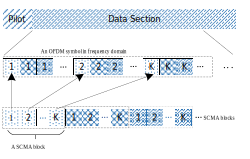
\includegraphics[width=0.45\textwidth]{Fig/Frams.pdf}  
% \caption{To be replaced} %最终文档中希望显示的图片标题
% \label{1} %用于文内引用的标签
% \end{figure}
 
 
%  \textbf { 3) CFO Estimation:}
%  After frame synchronization, the carrier frequency offset $\varepsilon$, which causes a phase rotation  % of $2\pi j \varepsilon_{R}/N$ 
% in the received signals,  is further to  be estimated. A training sequence based CFO estimation algorithm is exploited. Specifically, let $\mathbf r_{ss} = [r_{ss}(1),r_{ss}(2), \ldots, r_{ss}(N_{S}) ]^{\text{T}}$ denotes the received SS after frame synchronization and removing CP, then the  receiver makes the CFO estimation by utilizing the repetitive pattern of SS as follows \cite{zhang2005high,ZhangJoint}:
%  \begin{equation} 
%  \hat{\varepsilon }=\frac{1}{{2\pi }}\arg \sum \limits _{i = 0}^{ \frac{N_S}{2} - 1} {\left\lbrace {r_{ss}\left({i} \right) \text{conj} \left( r_{ss} \left({i+\frac{N_S}{2}} \right) \right)} \right\rbrace }. \end{equation}
 
%  Then,  the CFO for each OFDM symbol is corrected by multiplying $e^{-j2\pi \Delta_{f} i}, i = 1,2,\cdots, N_{S} $.
%  By using method proposed in \cite{zhang2005high} we know that $\varepsilon$ is conditionally unbiased, and given the high SNR, its estimation variance error can be approximated as
%  \begin{equation}
%  \label{cfo_err}
%  Var\left\{e_{\varepsilon}\vert\vert\varepsilon\vert<1\right\}\approx{1\over2\pi^{2}}\left[{1\over\eta}-\left(1+{1\over\eta}\right)\cdot e^{-\eta}\right],
%  \end{equation}
%  where $\eta=N_S\gamma^{2}/(4\gamma+2)$,  $\gamma$ is the received SNR and $e_{\varepsilon}$ is the estimation error of $ {\varepsilon }$.   
 
%   \textbf { 4) Channel estimation}: To estimate the distortion incurred by the channel and mitigate the effects of inter-symbol interference. The linear minimum mean square error (LMMSE) \cite{savaux2017lmmse,Edfors} algorithm is considered, which is expressed as 
%  \begin{equation}
% {{{ \hat{\bf{h}}}}_{LMMSE}} = {{{\bf R}}_{ {hh}}}{\left({{{{\bf R}}_{ {hh}}} +   \frac{\beta}{SNR}{{{\bf I}}_N}} \right)^{-1}}{{{\mathbf {x}_{ss}}}^{-1}}{{\mathbf r_{ss}}}, 
% \end{equation}
%  where   
%   \begin{equation}
%   \beta = E\lbrace {{{|{x}_{ss}(i)|}^2}}\rbrace E\lbrace {{{| {{1 / {x}_{ss}(i)}} |}^2}} \rbrace,
%  \end{equation}
%  is a constant depending on the transmitted signaling point, and    ${{{\bf R}}_{ {hh}}} = E \{\mathbf h \mathbf h^H\}$ is the  channel autocorrelation matrix.
 
 

% The transmit and receive antennas in the experiment experience a  strong LoS environment. Accordingly, the channel between each transmit-to-receive antenna pair can be characterized by Rician fading. %i.e., the channel can be expressed as 
% %  \begin{equation}
% % h{(i)} = \sqrt{\kappa \over \hbox{1} + \kappa} + \sqrt{\hbox{1} \over \hbox{1} + \kappa}\widetilde{h}{(i)}   
% %  \end{equation}
% %  where $\widetilde{h}{(i)} \sim {\cal CN}(\hbox{0}, \hbox{1})$ is a complex normal circular symmetric random variable with zero mean and unit variance and $ 1 \leq i \leq N_{S}$ is the  index of the subcarrier in an OFDM symbol.
% Similar to \cite{6525429,Zhang6733254}, the transmitter broadcasts pulses signal to measure channel environment,  and we obtain the channel environment followed a Rician distribution with $\kappa =30$. 
 
%   \textbf { 5) SNR Calculation:} Since each frame is consists of data section and zero section, the received signal in (\ref{downlink})  can be rewritten as 
%   \begin{equation}  \label{noise}
%  \mathbf{r}=  \left\{\begin{matrix}
%  \text{diag}\left( {{\mathbf{h}}} \right)\sum\limits_{j=1}^{J}{{{\mathbf{x}}_{j}}}+\mathbf{n}, & \text{data section,} \\ 
%  \mathbf{n}, & \text{zero section}.
% \end{matrix}\right.
% \end{equation} 
 
%  Then, proceeding from (\ref{noise}), we obtain 
%  \begin{equation}
%  \text{SNR}_{\text{dB}} = 10{\log _{10}}\frac{  E  \left \{ \left\Vert  \text{diag}\left( {{\mathbf{h}}} \right)\sum_{j=1}^{J}{{{\mathbf{x}}_{j}}} \right\Vert^2  \right \} }{{\sigma _n^2}},
%  \end{equation}
%  where 
%   \begin{equation}
%  \begin{aligned} 
%  \label{snr_tx} & E  \left \{ \left\Vert  \text{diag}\left( {{\mathbf{h}}} \right) \sum\nolimits _{j=1}^{J}{{{\mathbf{x}}_{j}}} \right\Vert  ^2  \right \} \\ &\quad\;= E  \left \{ {{\left\Vert {{\mathbf {r}}} \right\Vert ^2 - \left\Vert {{\mathbf {n}}} \right\Vert ^2 - 2{{ {{\mathbf {r}}} }^H}{\mathbf {n}}} } \right\},  \\
%  &\sigma _z^2 =  E \left\{ \left\Vert \mathbf{n} \right\Vert ^2 \right\} - E \left \{   \left\Vert \mathbf{n} \right\Vert \right\}^2.  \end{aligned}
%  \end{equation}

%  Note that in the practical system, the noise is including the AWGN noise and  thermal noise.  To obtain different SNR values at receiver, we change the value of  (\ref{snr_tx})  by tuning the power of transmit vectors.
 
 
\section{Numerical Results}

\begin{figure*}[htbp]
\centering
\subcaptionbox{$M=4$, $\lambda \in \left\{150\%, 200\%  \right\}$ and  $\text{E}_\text {b}/\text{N}_0 = 12$ dB \label{fig:Ex_Im}}{\includegraphics[width=0.44\textwidth]{Fig/awgn_Iter_v1-eps-converted-to.pdf}   } 
\subcaptionbox{$\lambda =150\%$, $M= 8$ ($\text{E}_\text {b}/\text{N}_0 = 14$  dB)  and $M= 16$ ($\text{E}_\text {b}/\text{N}_0 = 18$ dB) \label{fig:Ex_Im2}}{\includegraphics[width=0.44\textwidth]{Fig/awgn_Iter_M816_v1-eps-converted-to.pdf} }
\caption{Number of iterations vs. BER  performance of different codebooks ($\kappa \rightarrow \infty$). } \label{MPA_iter}
% \vspace{-5.5em}
\end{figure*}
%  \begin{figure*}[t] %H为当前位置,!htb为忽略美学标准,htbp为浮动图形
% \centering %图片居中
% \includegraphics[width=1\textwidth]{Fig/Complexity.pdf} %插入图片,[]中设置图片大小,{}中是图片文件名
% \caption{Normalized complexity comparison between different codebooks.} %最终文档中希望显示的图片标题
% \label{complexity}
%  \end{figure*}



In this section,  we conduct numerical evaluations of the proposed LPCBs for the $(4\times 6)$ and $(5\times 10)$ SCMA   systems characterized  in   (\ref{factor_46}) and (\ref{factor_510}), respectively.   These two systems lead to overloading factors of $\lambda =150\%$ and $\lambda = 200\%$ , respectively. 
Let $\text{A}_{M, T}$ denote  the proposed LPCB  of $M$-ary with $T$ LP numbers. Since the proposed permutation, labeling and sparse codebook optimization criteria are applicable in the   high  $\text{E}_\text{b}/\text{N}_0$ regime, we consider  $\text{E}_\text{b}/\text{N}_0 = 16$ dB, which is sufficiently large. In general, in an  IoT networks with an LoS path, a large $\kappa$ is assumed for many  scenarios \cite{5G_NR_s_iot, lutz1991land, vucetic1992channel,ErnestNOMA,WangTrajectory}. Hence, we set $\kappa = 20$ for the optimization of the proposed LPCBs. Moreover,
%As mentioned,  some constellation points in the proposed LPCB are overlapped in order to reduce the decoding complexity, thus the diversity between these constellation pairs are sacrificed. Therefore,  we give more room to maximize  ${\Theta}_{\min}^{   \mathbf {\mathcal X}_{\lambda,M,T}}$ and set $\kappa = 15$ dB  during optimization.
considering the trade-off between the computation complexity and accuracy, we set $Q=10000$ and $t_{\text{max}}=20$ for the cases of $M \geq 16$ or $\lambda = 200\%$.  The details of the designed LPCBs   are given in  our GitHub project\footnote{\url{https://github.com/ethanlq/SCMA-codebook}} and some LPCBs are also presented in Appendix C.




The main  state-of-the-art  codebooks for comparison with the proposed ones are the GAM codebook \cite{mheich2018design}  and the Star-QAM codebook \cite{yu2015optimized}\footnote{We have also optimized the MCs  that proposed  in \cite{bao2017bit} with the proposed design approach. However, it is found that the resultant BER performance is far in ferier to the GAM and Star-QAM codebooks in downlink channels. }. 
 This is because  both  \cite{mheich2018design} and \cite{yu2015optimized}   achieve  good BER performance in downlink channels. %In addition, the  state-of-the-art codebooks proposed in \cite{chen2020design} and  \cite{huang2021downlink},  denoted respectively as Chen and Huang codebook, are also employed for comparison.
 We first analyze  and present the complexity reduction of our  proposed LPCBs for MPA decoder. Then, the BER performances  are  compared with  the benchmark codebooks in both uncoded and coded systems. %Finally, we evaluate our proposed codebooks in a hardware prototype based on an USRP.  
  \begin{table}[]
  \small
 \centering
 \caption{Comparison of the proposed codebooks in terms of $\Delta_{\min}$,  MED and $I_t$. }
     \begin{tabular}{c|c|c|c|c}
    \hline
    \hline
       \makecell[c] {System setting \\ ($M,\lambda$)}    &  Codebooks & $\Delta_{\min}$  & MED & \makecell[c] {$I_t $  (MPA)} \\
    \hline
    \hline
    \multirow{4}{*}{$\left(4, 150\% \right)$} & $\text{A}_{4,2}$ & 1.16 & 1.1 & 1 \\
    \cline{2-5}
    &$\text{A}_{4,3}$ & 1.31 & 1.23 & \multirow{4}{*}{$ 4$}\\
    \cline{2-4}
    & Star-QAM  \cite{yu2015optimized}& 0.98 & 0.9   \\
    \cline{2-4}
     & GAM \cite{mheich2018design}   & 0.74  & 0.57  \\
   \cline{2-4}
    & Huawei \cite{huawei} & 0.67  & 0.57    \\
    % \cline{2-4}
    %  & Chen \cite{chen2020design} & 1.14  & 1.07     \\
    %      \cline{2-4}
    %       & Huang \cite{huang2021downlink} & 1.36  & 1.30     \\
    \hline
    \hline
    \multirow{4}{4em}{$\left(4, 200\% \right)$} & $\text{A}_{4,2}$ & 1.05 & 0.96 & $ 1$\\
    \cline{2-5}
    &$\text{A}_{4,3}$ & 0.75 & 0.64 & $ 4$ \\
    \cline{2-5}
    & Star-QAM \cite{yu2015optimized}& 0.56 & 0.48 &\multirow{2}{*}{$ 6 $}\\
    \cline{2-4}
     & GAM \cite{mheich2018design} & 0.47 & 0.43 \\
    \hline
    \hline
    \multirow{4}{4em}{$\left(8, 150\% \right)$} & $\text{A}_{8,3}$& 0.62 & 0.54 & $2$\\
    \cline{2-5}
    &$\text{A}_{8,4}$ & 0.75 & 0.67 & $ 4$ \\
    \cline{2-5}
    &$\text{A}_{8,5}$& 0.62 & 0.53 & $ 4$ \\
    \cline{2-5}
    &$\text{A}_{8,6}$ & 0.51 & 0.46 & $ 5$ \\
    \cline{2-5}
    &$\text{A}_{8,7}$& 0.54 & 0.50 & $ 5$ \\
    \cline{2-5}
    & Star-QAM \cite{yu2015optimized}& 0.5 & 0.45   & $4$\\
    \cline{2-5}
     & GAM \cite{mheich2018design} & 0.51 & 0.47 & $6$\\
    \hline
    \hline     
    \multirow{4}{*}{$\left(16, 150\% \right)$} & $\text{A}_{16,4}$ & 0.32  & 0.26 & $ 1$\\
    \cline{2-5}
    &$\text{A}_{16,9}$&   0.28 &   0.21  & $ 5$ \\
    \cline{2-5}
    & Star-QAM \cite{yu2015optimized}& 0.2 & 0.15 &  $7 $  \\
    \cline{2-4}
     & GAM \cite{mheich2018design}  & 0.2 & 0.16 & $7 $\\
    \hline
     \end{tabular}
     \label{codebooks}
 \end{table}

%  \begin{table}[]\small
%  \centering
%  \caption{Comparison of proposed codebooks in terms of $\Delta_{\min}$,  MED and complexity reduction }
%      \begin{tabular}{c|c|c|c|c}
%     \hline
%     \hline
%       \makecell[c] {System scale \\ ($M,\lambda$)}    &  Codebooks & $\Delta_{\min}$  & MED & \makecell[c] {Complexity \\ Reduction } \\
%     \hline
%     \hline
%     \multirow{4}{*}{$\left(4, 150\% \right)$} & $\text{A}_{42}$ & 1.16 & 1.1 & $58 \%$\\
%     \cline{2-5}
%     &$\text{A}_{43}$ & 1.31 & 1.23 & $ 87\%$ \\
%     \cline{2-5}
%     & Star-QAM  & 0.98 & 0.9 & \multirow{4}{*}{$0 $}  \\
%     \cline{2-4}
%      & GAM  & 0.74  & 0.57  \\
%   \cline{2-4}
%     & Huawei \cite{huawei} & 0.67  & 0.57    \\
%     \cline{2-4}
%      & Chen \cite{chen2020design} & 1.14  & 1.07     \\
%     \hline
%     \hline
%     \multirow{4}{4em}{$\left(4, 200\% \right)$} & $\text{A}_{42}$ & 1.05 & 0.96 & $ 94\%$\\
%     \cline{2-5}
%     &$\text{A}_{43}$ & 0.75 & 0.64 & $ 68\%$ \\
%     \cline{2-5}
%     & Star-QAM & 0.56 & 0.48 &\multirow{2}{*}{$0 $}\\
%     \cline{2-3}
%      & GAM & 0.47 & 0.43 \\
%     \hline
%     \hline
%     \multirow{4}{4em}{$\left(8, 150\% \right)$} & $\text{A}_{83}$& 0.62 & 0.54 & $95\%$\\
%     \cline{2-5}
%     &$\text{A}_{84}$ & 0.75 & 0.67 & $ 87\%$ \\
%     \cline{2-5}
%     &$\text{A}_{85}$& 0.62 & 0.53 & $ 76\%$ \\
%     \cline{2-5}
%     &$\text{A}_{86}$ & 0.51 & 0.46 & $ 58\%$ \\
%     \cline{2-5}
%     &$\text{A}_{87}$& 0.54 & 0.5 & $ 33\%$ \\
%     \cline{2-5}
%     & Star-QAM & 0.5 & 0.45   &\multirow{2}{*}{$0 $}\\
%     \cline{2-4}
%      & GAM & 0.51 & 0.47 \\
%     \hline
%     \hline     
%     \multirow{4}{*}{$\left(16, 150\% \right)$} & $\text{A}_{164}$ & 0.32  & 0.26 & $ 98\%$\\
%     \cline{2-5}
%     &$\text{A}_{169}$&   0.28 &   0.21  & $ 82\%$ \\
%     \cline{2-5}
%     & Star-QAM & 0.2 & 0.15 & \multirow{2}{*}{$0$}  \\
%     \cline{2-4}
%      & GAM & 0.2 & 0.16 \\
%     \hline
%      \end{tabular}
%      \label{codebooks}
%  \end{table}




Table \ref{codebooks} compares  the  $\Delta_{\min}$  of the proposed  codebooks, GAM and Star-QAM for the  SCMA  systems with overloading $\lambda =150\%$ and $\lambda = 200\%$, respectively. In addition, since the MED is widely used as a performance metric, we also present the MED of different codebooks. 
Clearly, most of the proposed LPCBs enjoy larger $\Delta_{\min}$ and MED values. % To the authors’ best knowledge,  for ($\lambda =150\%$) SCMA setting, the codebook reported in \cite{huang2021downlink} owns the largest MED value  among all existing codebooks.  One can see our proposed  $\text{A}_{4,3}$ codebook only  slightly smaller than that of \cite{huang2021downlink}. In addition,  $\text{A}_{4,3}$ has the distinct feature of  LP numbers which  can reduce the decoding complexity.
For example,  the  MEDs of proposed codebooks $\text{A}_{4,3}$ and $\text{A}_{4,2}$ of $\lambda =150\%$ and $\lambda = 200\%$ SCMA systems, respectively,  are significantly larger than that of other codebooks. %
 It is also  worth mentioning that, to our   best knowledge, the proposed codebooks $\text{A}_{4,2}$ for  $ \lambda = 150\%$,    $\text{A}_{8,4 }$ and $\text{A}_{16,4}$ for $ \lambda = 200\%$,  enjoy the largest  MED values  among all existing codebooks. 


  
\subsection{Complexity reduction of MPA with the  proposed LPCBs}  
In this subsection, we evaluate the  convergence behaviors of MPA  with the proposed LPCBs  and compare the receiver complexities of the proposed LPCBs with conventional codebooks  \cite{mheich2018design,yan2016top,deka2020design,yu2015optimized,klimentyev2017scma,Zhang,li2020design,chen2020design}, referred as Non-LPCBs.  

\begin{figure*}[htbp]
	\centering
	\begin{subfigure}{0.24 \textwidth}
  \includegraphics[width=1.1 \linewidth]{{Fig/complexity_1-eps-converted-to.pdf}}
		\caption{$\lambda =150\%$, $M= 4$  }
				\vspace{-0.1em}
	\end{subfigure}
	\begin{subfigure}{0.24\textwidth}
  \includegraphics[width=1.1 \linewidth]{{Fig/complexity_2-eps-converted-to.pdf}}
		\caption{$\lambda =150\%$, $M= 8$  }
		\vspace{-0.1em}
	\end{subfigure}
	\begin{subfigure}{0.24 \textwidth}
  \includegraphics[width=1.1 \linewidth]{{Fig/complexity_3-eps-converted-to.pdf}}
		\caption{$\lambda =150\%$, $M= 16$  }
				\vspace{-0.1em}
	\end{subfigure}
	\begin{subfigure}{0.24\textwidth}
  \includegraphics[width=1.1 \linewidth]{{Fig/complexity_4-eps-converted-to.pdf}}
		\caption{$\lambda =200\%$, $M= 4$  }
		\vspace{-0.1em}
	\end{subfigure}	
	\caption{Complexity reduction of the proposed LPCBs with MPA.}
	\label{complexity}
	\vspace{-1.5em}	
\end{figure*}
 \begin{figure*} 
\centering
\subcaptionbox{$M=4$ and $\lambda \in \left\{150\%, 200\%  \right\}$ \label{fig:Ex_Im}}{\includegraphics[width=0.42\textwidth]{Fig/awgn_m4_v1-eps-converted-to.pdf}  } 
\subcaptionbox{$\lambda =150\%$ and $M \in \left\{8, 16 \right\}$ \label{fig:Ex_Im2}}{\includegraphics[width=0.42\textwidth]{Fig/awgn_m816_v1-eps-converted-to.pdf}}
\caption{BER performance of different codebooks   with $\kappa \rightarrow \infty$.}
\label{BER_AWGN}
\end{figure*}
 \begin{figure*}
\centering
\subcaptionbox{$M=4$, $\lambda \in \left\{150\%, 200\%  \right\}$   \label{fig:Ex_Im}}{\includegraphics[width=0.42\textwidth]{Fig/rician_m4_v1-eps-converted-to.pdf}   } 
\subcaptionbox{$\lambda =150\%$ and $M \in \left\{8, 16 \right\}$ \label{fig:Ex_Im2}}{\includegraphics[width=0.42\textwidth]{Fig/rician_m816_v1-eps-converted-to.pdf} }
\caption{BER performance of different codebooks     with $\kappa= 15$. }\label{BER_rician}
	\vspace{-1.5em}	
\end{figure*}

We first present  the convergence behaviors of different codebooks with $\kappa \rightarrow \infty$ of MPA decoder in Fig. \ref{MPA_iter}.    The number of iterations $I_t$ for decoding convergence of different codebooks are also summarized in Table \ref{codebooks}.
It is noted that most of the proposed codebooks enjoy   faster convergence rate  than the Star-QAM codebook and GAM codebook\footnote{For other values of $\kappa$, we also observe the same result that the proposed LPCBs require less iterations for convergence.}. With reduced  projected numbers ($T$), less message  propagation  between function nodes and variable nodes are required  during MPA iteration, thus leading to less iterations for convergence.  
In particular,   the proposed codebooks $\text{A}_{4,2}$,  $\text{A}_{8,3}$ and  $\text{A}_{16,4}$ for $\lambda = 150\%$,  and $\text{A}_{4,2}$ for $\lambda = 200\%$ only need about one iteration to converge. The decoding can be carried out in a one-shot for these codebooks and the decoding complexity is significantly reduced compared to other codebooks.   

 The computation complexity  in terms of multiplication  and addition of   MPA  can be approximated as \cite{yang2016low,bayesteh2015low}:
\begin{equation} 
\small
\begin{aligned}
&{N_{m}} = [({d_{f}} + 3){T^{d_{f}}}{N} \! + \! ({N} \!- \!2)T{N}]J{I_{t}} + T({N} - 1)J,\\ 
&{N_{a}} 
=[({d_{f}}\! + \!1){T^{d_{f}}}{N} \! +\!  (T \!- \!1){N}{\mathrm{ + (}}{T^{d_f \!- \! 1}} \!-\! 1)T{N}]J{I_{t}},  \\  \end{aligned}
\end{equation}
respectively. Clearly,  the decoding complexity depends on  $T$, $I_{t}$ and the system overloading.     To proceed, we further define the   complexity reduction ratio (CRR) as follows \cite{bao2017bit}:
 \begin{equation}
 \small
     \text{CRR} \triangleq 1- \frac{\text{Number of Operations of LPCBs}}{\text{Number of Operations of Non-LPCBs}}.
 \end{equation}
  
As shown in Fig. \ref{complexity}, it is evident that the proposed LPCBs can greatly reduce the detection complexity, with  more than about $60\%$ complexity reduction being achieved compared to Non-LPCBs.  
The gain becomes more significant  as the increase of $M$ and  $\lambda$.   For example, the proposed codebooks  $\text{A}_{8, 3}$ and $\text{A}_{16,4}$ can reduce the decoding complexity by $97.4\%$ and $99.8\%$, respectively.  


 \begin{figure*}[htbp]
\centering
\subcaptionbox{$M=4$ and $\lambda =150\%  $ \label{fig:Ex_Im}}{\includegraphics[width=0.44\textwidth]{Fig/F46_LDPC_M4_v1-eps-converted-to.pdf}     } 
\subcaptionbox{$M=8$ and $\lambda =150\%  $ \label{fig:Ex_Im2}}{\includegraphics[width=0.44\textwidth]{Fig/F46_LDPC_M8_v1-eps-converted-to.pdf}   }
\subcaptionbox{$M=16$ and $\lambda =150\%  $ \label{fig:Ex_Im}}{\includegraphics[width=0.44\textwidth]{Fig/F46_LDPC_M16_v1-eps-converted-to.pdf}      } 
\subcaptionbox{$M=4$ and $\lambda =200\%  $ \label{fig:Ex_Im2}}{\includegraphics[width=0.44\textwidth]{Fig/F510_LDPC_M4_v1-eps-converted-to.pdf}   }
\caption{LDPC coded BER performance comparison of different  codebooks.}\label{CodedBER}
\end{figure*}




\subsection{Comparison of uncoded BER performance}



In this subsection, we evaluate the uncoded BER performance of the proposed  LPCBs.  
    $\kappa \rightarrow \infty$ is the typical value for open environments in satellite IoT \cite{5G_NR_s_iot}. In the rural and suburban scenarios of satellite IoT, and UAV IoT networks,   large  $\kappa$  is  generally assumed \cite{lutz1991land, vucetic1992channel,ErnestNOMA}.    Hence, we consider  $\kappa \rightarrow \infty$ and $\kappa  = 15$ for the uncoded systems, which are shown in Fig. \ref{BER_AWGN} and  Fig. \ref{BER_rician}, respectively.  
% we consider  the  5G new radio (NR) satellite   channel model, as specified in TR 38.811 \cite{5G_NR_s_iot}. According to \cite{5G_NR_s_iot}, the typical   $\kappa$ values for open,  rural, suburban and dense urban environments are given as $\kappa \rightarrow \infty$, $\kappa = 40$, $ 12\leq \kappa \leq 22$ and  $   \kappa =12$, respectively.
%To further demonstrate the superiority of proposed codebooks in terms of MED and investigate the convergence behavior with MPA, we conduct BER simulation in AWGN channel, which.
   As can be seen in Fig. \ref{BER_AWGN}, the proposed codebook  $\text{A}_{4,3}$   for $\lambda = 150\%$ achieves about $2$ dB gain over the Star-QAM codebook and $4$ dB gain over the GAM codebook at BER = $10^{-5}$, respectively. Moreover,   $\text{A}_{4,3}$   for $\lambda =200\%$ also outperforms  than  the Star-QAM codebook and the GAM codebook. The excellent BER advantage  can be observed for the proposed   $\text{A}_{4,2}$  codebook for $\lambda = 200\%$ due to large MED, which achieves about $3$ dB gain over the Star-QAM codebook and $4.5$ dB gain over the GAM codebook at BER=$10^{-5}$, respectively. For $M \in \left\{8, 16 \right\}$ and $\lambda =150\%$, we are interested in   codebooks with less projected numbers, thus only $\text{A}_{8,3}$, $\text{A}_{8,4}$ and $\text{A}_{8,5}$ are compared to GAM and Star-QAM codebooks in Fig. \ref{BER_AWGN}(b). One can see that  the proposed codebooks outperform the GAM and Star-QAM codebooks significantly. Among these codebooks, $\text{A}_{8,4}$ and $\text{A}_{16,4}$ achieve the best BER performance for $M=8$ and $M=16$, respectively.  In particular,  $\text{A}_{8,4}$  has a gain about $3.8$ dB over the GAM codebook and $4.2$ dB over  the Star-QAM codebook, respectively.

From Fig. \ref{BER_rician},   we have the following main observations: 1) For the case of $\kappa  = 15$, most of the proposed  LPCBs   achieve good BER performance. In particular, the codebooks $\text{A}_{4,3}$ ($\lambda =150\%$), $\text{A}_{4,2}$ ($\lambda =200\%$), $\text{A}_{8,4}$ still outperform the GAM and Star-QAM codebooks;  2) Compared with the results in  Fig. \ref{BER_AWGN}, the performance of  LPCBs with smallest LP numbers for  $\kappa  = 15$, such as $\text{A}_{4,2}$ ($\lambda =150 \%$),  $\text{A}_{8,3}$, $\text{A}_{16,4}$  are more likely affected  by the channel fading.



\subsection{Comparison of coded BER performance}

 \begin{table}  
\small
    \caption{Simulation Parameters}
    \centering
    \begin{tabular}{c|c}
    \hline
     \hline
       \textbf{ Parameters}  &  \textbf{ Values}  \\
        \hline
         \hline
       Transmission  &  Downlink \\
        \hline
       Channel model  &  Rician fading channel, $\kappa =2, 30$ \\
        \hline
        SCMA setting & $\lambda = 150\%$ and $\lambda = 200\%$ \\
          \hline
        Channel coding &  \makecell[c] {5G NR LDPC codes with \\ rate  of $0.8462$ and block length of $260$ }  \\ 
         \hline
        Codebooks &  \makecell[c] {The same codebooks presented in  \\ Fig. \ref{BER_AWGN} and Fig. \ref{BER_rician} }  \\ 
       \hline
       Receiver &   \makecell[c] { Turbo-MPA: \\ $1$ MPA iteration  for  $\text{A}_{4,2}$ ($\lambda = 150\%$), \\ $\text{A}_{4,2}$ ($\lambda = 200\%$), $\text{A}_{8,3}$ and $\text{A}_{16,4}$, \\and $4$ MPA iterations for other codebooks, \\ 5 BICM iterations } \\
         \hline
    \end{tabular}
    \label{sim_para}
    \vspace{-1.5em}
\end{table}
 

In this subsection, we compare the coded BER performances of the    proposed codebooks with the GAM   and Star-QAM codebooks.  In some scenarios, such as   dense urban and urban areas with an LoS path,      $\kappa$ is relatively small \cite{5G_NR_s_iot, lutz1991land, vucetic1992channel}. Hence, we set  $\kappa$ with a wide range. Considering  the short-packet nature of IoT networks, we apply the 5G NR LDPC codes with small block length \cite{liu2021sparse,PerturbedDeng}, as specified in TS38.212 \cite{5G_NR}.  The detailed simulation settings are  given in Table \ref{sim_para} and the simulated   BER performance   are depicted in Fig. \ref{CodedBER}.

In Fig. \ref{CodedBER}(a), the proposed codebook $\text{A}_{4,2}$ and  $\text{A}_{4,3}$  show  better performance than the GAM and Star-QAM codebooks for $\kappa = 30$. In particular, the  $\text{A}_{4,3}$ outperforms Star-QAM codebook by $1$ dB gain at BER$=10^{-4}$. When there exists severe fading, i.e., $\kappa =2$, the error performance  of $\text{A}_{4,2}$ deteriorates, however, the  proposed $\text{A}_{4,3}$ still achieves similar BER performance with the Star-QAM codebook and performs  slightly better in the low $E_b/N_0$ range. By observing the slopes   of the curves, the GAM codebook enjoys a larger   diversity gain than the low projected codebooks.  This is because some constellation points in the LPCBs are overlapped in order to reduce the decoding complexity, thus the diversity between these constellation pairs may be reduced.   However, we show that by properly designing the MC and maximising the coding gain, most of the proposed LPCBs  can still achieve good   BER performance for $\kappa =2$.   


For the    $8$-ary and $16$-ary  codebooks shown in Fig.  \ref{CodedBER}(b) and Fig.  \ref{CodedBER}(c), respectively, BER trends similar to that of the $4$-ary codebook are observed.   The proposed   codebooks outperform  the GAM  and Star-QAM codebooks for  $\kappa=30$, whereas the error  performance of the  proposed codebooks with   least projection numbers  deteriorate  for the case of $\kappa =2$.  
It is interesting to  see the proposed codebook $\text{A}_{8,4}$ and $\text{A}_{16,4}$ achieve the best coded BER performance for both  $\kappa=30$ and  $\kappa=2$ among all the codebooks owing to the well optimized bit labeling   and large coding gain. For example, $\text{A}_{8,4}$ achieves about $3.6$ dB gain over the GAM codebook and $1.5$ dB gain over the Star-QAM  codebook for $\kappa=30$,  and   achieves about $2$ dB gain over the GAM codebook and $1$ dB gain over the Star-QAM  codebook for $\kappa=2$ at BER$=10^{-4}$, respectively.
 
 As shown in Fig.  \ref{CodedBER}(d), for the  SCMA system with $\lambda = 200\%$,   the proposed codebook $\text{A}_{4,2}$ achieves about $1$ dB gain compared to the GAM with $\kappa = 30$ due to the very large coding gain, however, the BER curve degrades   earlier than others for    $\kappa=2$. The  superiority of  the proposed codebooks mainly   lies in  the huge reduction of complexity, especially in largely  overloaded system.
 

 
% \subsection{Over the air performance of proposed codebooks}

% In this subsection,  we  seek to characterize the performance of SCMA with an experimental testbed. We occupy OFDM waveform  for SCMA transmission, and  evaluate the performance of our proposed codebooks in OFDM-SCMA  with SDR. The National Instruments (NI) PXIe device,   universal software radio peripheral (USRP)  software defined radios (RIOs) and  CDA-1990 clock  are used for the system prototype.  LabVIEW communications system design suite \footnote{LabVIEW Communications system design suite is designed special for prototyping of  wireless communications systems  to validate wireless algorithms with over-the-air (OTA) signals using a unified graphical programming approach.} is used for the software programming. 

% %The prototype testbed setup for  the downlink SCMA system is illustrated in Fig 5 (to be addded).
% Regarding the environments, the transmitter (Tx) is placed in an indoor environment with a height of $0.7$m.    The receiver (Rx) is placed at distances of $2$m from the Tx with heights $0.7$m.    The data to be transmitted are first processed at TX-PXIe, including SCMA modulation, OFDM modulation and framing. Then, the time domain  data  are  transmitted by USRP-RIO1 through its radio channel. At the receiver, the USRP-RIO2  records the  sampled data and delivery the data to RX-PXIe for real-time processing. The receiver  consists of timing synchronization module, carrier frequency offset (CFO) correction, OFDM demodulation, channel estimation, SNR calculation, SCMA demodulation and BER calculation units.   
%  A training sequence with  the length of FFT size is employed for synchronization,  CFO estimation and channel estimation.  The linear minimum mean square error (LMMSE) \cite{savaux2017lmmse,Edfors} algorithm is considered for channel estimation. Specifically, the channel is estimated at the beginning of each frame for both Tesdbed and  simulation, and we assume the channel remains unchanged for each frame in the simulation. The transmit and receive antennas in the experiment experience a  strong LoS environment. Accordingly, the channel between each transmit-to-receive antenna pair can be characterized by Rician fading.  
% Similar to \cite{6525429,Zhang6733254}, the transmitter broadcasts pulses signal to measure channel environment,  and we obtain the channel environment followed a Rician distribution with $\kappa =30$.
%  To attain frequency diversity for an OFDM-SCMA system,  it requires to provide as much separation as possible when mapping the SCMA resources within a block to the OFDM subcarriers.    Therefore, we propose to allocate the transmitted symbols within a SCMA block to an OFDM symbol in a separate manner, denote as \textit{separate allocation}.   The detailed implementation parameters for the Testbed are given in Table \ref{testbed}.  For more detailed implementation, please refer to our  source code  at our GitHub project \footnote{xxxxxx.}.  
%   \begin{table} \small
%  \centering
%  \caption{Testbed parameters}
%      \begin{tabular}{c|c}
%      \hline
%     Parameters & Values\\
%     \hline
%      Transmission  & SCMA downlink transmission \\
%      SCMA systems      & $\lambda =150\%, 200\%$ and $M=4$  \\
%      Resource allocation &  Separate allocation\\
%      Decoder     &  Log-MPA \\
%      Channel estimation & LMMSE\\
%      Codebooks   &  $A_{42}$, $A_{43}$, Huawei, Star-QAM\\
%           FFT length ($N_S$)     & $64$ \\
%           CP length    & $\frac{1}{16} N_S$  \\
%          \makecell[c]  {Number of OFDM \\ symbols per frame} & 30\\
%           Training sequence  length & $N_S$\\
%           Frame length & 2108 \\
%           Subcarrier spacing & $15$ kHz \\
%           Central frequency & $2.4$ Ghz \\
%   \hline
%      \end{tabular}
%      \label{testbed}
%  \end{table}
% %   \begin{figure}[] %H为当前位置,!htb为忽略美学标准,htbp为浮动图形
% % \centering %图片居中
% % \includegraphics[width=0.4\textwidth]{Fig/Test-eps-converted-to.pdf}  
% % \caption{ Uncoded BER performance comparison of measured   and simulation results for $M=4$  in ($5\times10$) SCMA systems.} %最终文档中希望显示的图片标题
% % \label{Testbed_F510_M4} %用于文内引用的标签
% %  \end{figure}
% \begin{figure}[] %H为当前位置,!htb为忽略美学标准,htbp为浮动图形
% \centering %图片居中
% \includegraphics[width=0.5\textwidth]{Fig/TestbedF46-eps-converted-to.pdf}  
% \caption{ Uncoded BER performance comparison of measured   and simulation results for $M=4$  in ($4\times6$) SCMA systems.} %最终文档中希望显示的图片标题
% \label{Testbed_F46_M4} %用于文内引用的标签
%  \end{figure}
%  \begin{figure}[] %H为当前位置,!htb为忽略美学标准,htbp为浮动图形
% \centering %图片居中
% \includegraphics[width=0.5\textwidth]{Fig/TestbedF510-eps-converted-to.pdf}  
% \caption{ Uncoded BER performance comparison of measured   and simulation results for $M=4$  in ($5\times10$) SCMA systems.} %最终文档中希望显示的图片标题
% \label{Testbed_F510_M4} %用于文内引用的标签
%  \end{figure}


% We  now present the simulation and experimental results for  Huawei codebook,   Star-QAM codebook and  proposed codebooks  in an indoor environment. 
% Fig. \ref{Testbed_F46_M4} and Fig. \ref{Testbed_F510_M4}  show  the simulation  and measured results of different codebooks in $\lambda = 150\%$ and $\lambda = 200\%$ SCMA systems, respectively.  
% A large error  between the experimental and simulation curves is observed at low BER ranges in Fig. \ref{Testbed_F46_M4} and Fig. \ref{Testbed_F510_M4}. This can be attributed to a number of factors, including incorrect FO estimation, poor channel estimation, timing recovery errors and synchronization problems. As the  $\text{E}_\text{b}/\text{N}_0$ increases, however, CFO estimation, timing recovery, and channel estimation improve, leading to a lower BER. The difference between measured and simulation results are mainly attributed to the hardware imperfections, such as the RF channel correlation, power amplifier   non-linearity, phase noise, and IQ imbalance\footnote{The USRP RIO adopt the low cost zero intermediate frequency   RF architecture, and the inherent of such architecture is the effect of IQ imbalance, which may degrades the BER performance. Moreover, due to the slight differences % due to variances
% in hardware components, temperature, and other factors, the I and Q signal path are subject to different conditions, which may also result in the IQ imbalance.}.
% Overall, the proposed codebooks achieve good BER performance in the real indoor environment due to the large MED values, especially for the codebooks $\text{A}_{4,3}$ and $\text{A}_{4,2}$ of $\lambda = 150\%$ and $\lambda = 200\%$ SCMA systems, respectively. It is also worth to mentioning that the proposed codebook can significantly reduce the decoding complexity of MPA or Log-MPA.


\section{Conclusion}
 
In this paper,  we have  introduced a novel  class of SCMA codebooks that  can significantly reduce the decoding complexity  while achieving  good BER performance
  for downlink IoT networks.  We    have analyzed  the corresponding pairwise  error probability   of SCMA transmissions under a generalized  Rician fading channel model and derived the codebook design criteria.   To reduce the decoding complexity, we have proposed to construct the MC with LP-GAM by allowing several overlapped constellation points in each dimension.   In addition, we have developed     an  efficient  codebook design approach, including permutation, bit labeling, sparse codebook construction and parameter optimization. 
Numerical results demonstrated the  benefits of proposed codebook in terms of complexity reduction and BER performance improvements in different  IoT  environments. In particular, some codebooks (e.g., $\text{A}_{4,2}$, $\text{A}_{4,3}$, $\text{A}_{8,4}$ and $\text{A}_{16,4}$ for   $ \lambda = 150\%$ system  and $\text{A}_{4,2}$ for $ \lambda = 200\%$ system ) achieve significant performance improvements for typical $\kappa $ values in  open, rural and suburban environments,  and significant complexity reduction compared  to the existing codebooks.
%Finally, to experimentally validate the BER performance of downlink SCMA system, a hardware platform based on SDR was implemented.   The measured results also demonstrate the benefits of proposed codebooks.



 
 
 
 



% if have a single appendix:
%\appendix[Proof of the Zonklar Equations]
% or
%\appendix  % for no appendix heading
% do not use \section anymore after \appendix, only \section*
% is possibly needed

% use appendices with more than one appendix
% then use \section to start each appendix
% you must declare a \section before using any
% \subsection or using \label (\appendices by itself
% starts a section numbered zero.)
%


 \appendices
\section{Proof of the Lemma 1} 
\label{AppeA}
\textit{1). }   For  $(1+\kappa) \gg \frac{ \tau _{{{\mathbf w}} \rightarrow {\tilde{\mathbf{w}}}}(k)  }{4N_0}$, we have 
  \begin{equation}
   \small
  \label{d_awgn}
d_{1, \mathbf{w} \to \mathbf{\hat{w}} }^2(k) = \frac{\kappa \tau _{{{\mathbf w}} \rightarrow {\tilde{\mathbf{w}}}}(k) }{\kappa +1}, d_{2, \mathbf{w} \to \mathbf{\hat{w}} }^2(k)=0,
    \end{equation}
and thus $d_{ \mathbf{w} \to \mathbf{\hat{w}} }^2 = \frac{\kappa \delta_{{{\mathbf w}} \rightarrow {\tilde{\mathbf{w}}}}}{1+\kappa}$. In this special case, (\ref{PEP_Raician2})   reduces to 
\begin{equation}
 \small
 \label{PEP_awgn}
\begin{aligned} 
\text{Pr} \{\mathbf{w} \to \mathbf{\hat{w}}\}   \leq  \exp \left(-\frac{\kappa \delta_{{{\mathbf w}} \rightarrow {\tilde{\mathbf{w}}}}}{4\left( 1+\kappa \right)N_0}\right).
\end{aligned}
  \end{equation}
  
Then, based on  (\ref{ABER}) and  (\ref{PEP_awgn}) , we know that the ABER is dominated by the  MED  between $ \mathbf {w} $ and $\hat {\mathbf {w}}$ in $\Phi _{M^J}$, which corresponding to the MEEs that  all the errors occurred with multiple users.  Therefore,   an important codebook design criteria in this case   is  to  maximize  the MED of the superimposed codewords, which has been widely employed  for SCMA systems operating in the   AWGN channel \cite{klimentyev2017scma,huang2021downlink,li2020design}.  Note that the MED can also obtained by letting   $\kappa \rightarrow \infty$ in $ {{\Delta}_{\min} \left( { \boldsymbol {\mathcal X}} \right)}$. 
      
      
      
\textit{2). } In the case when   $(1+\kappa) \ll \frac{ \tau _{{{\mathbf w}} \rightarrow {\tilde{\mathbf{w}}}}(k)  }{4N_0}$,  we have
  \begin{equation}
   \small
  \label{dRay}
d_{1, \mathbf{w} \to \mathbf{\hat{w}} }^2(k) =4N_0 \kappa, d_{2, \mathbf{w} \to \mathbf{\hat{w}} }^2(k)= 4N_0   \ln \left(- \frac{{  \tau _{{{\mathbf w}} \rightarrow {\tilde{\mathbf{w}}}}(k)  }  }{4N_0 \left( 1+ \kappa\right)}   \right),
    \end{equation}
and thus $d_{ \mathbf{w} \to \mathbf{\hat{w}} }^2$ is the sum of the logarithms of the element-wise distance. 
% To proceed, let us define
%   \begin{equation}
%     \small
%   \begin{aligned} & D (\mathbf {w}\rightarrow \hat {\mathbf {w}}) \triangleq\left \{{k: \tau _{{{\mathbf w}} \rightarrow {\tilde{\mathbf{w}}}}(k)\neq 0, 1\leq k \leq K }\right \}, \\ 
%   & G_{d} (\mathbf {w}\rightarrow \hat {\mathbf {w}})\triangleq \sum \limits _{k=1}^{K}\text {Ind}\left (\tau _{{{\mathbf w}} \rightarrow {\tilde{\mathbf{w}}}}(k)\right), 
%   \end{aligned}
%   \end{equation}
% where $\text {Ind}(x)$ takes the value of one if $x$ is nonzero and zero otherwise. Clearly, $G_{d} (\mathbf {w}\rightarrow \hat {\mathbf {w}})$ gives the cardinality of set $D(\mathbf {w}\rightarrow \hat {\mathbf {w}})$.
Substituting (\ref{dRay}) and (\ref{d}) into (\ref{PEP_Raician2}), we obtain the PEP   for this special   case as 
    \begin{equation}
\label{PEP_rayleigh}
 \small
\begin{aligned} 
 \small
\text{Pr} \{\mathbf{w}\! \to \!\mathbf{\hat{w}}\}   \leq 
 {\prod \limits _{k \in D (\mathbf {w}\rightarrow \hat {\mathbf {w}})}  \! \left( \frac{   \tau _{{{\mathbf w}} \rightarrow {\tilde{\mathbf{w}}}}(k)   }{4N_0\left(1+\kappa\right)}  \right)^{-1} \!
 {\exp \left(- \kappa \right) }}. 
\end{aligned}
  \end{equation}
where $ D (\mathbf {w}\rightarrow \hat {\mathbf {w}})$ denotes the     set of  indices in which $ \tau _{{{\mathbf w}} \rightarrow {\tilde{\mathbf{w}}}}(k)   \neq 0$.
Note  that one can approximate the right-hand side of (\ref{PEP_rayleigh})  as  
 \begin{equation}
  \small
 \label{pep_gcgd}
\text{Pr} \{\mathbf{w} \!\to \!\mathbf{\hat{w}}\} \leq
G_{c} \left(\mathbf {w} \! \rightarrow \!\hat{\mathbf {w}} \right) \!
  \left (\frac {1}{ 4N_0 \left(1\!+\! \kappa\right)} \right)^{-{G_{d} (\mathbf {w}\rightarrow \hat {\mathbf {w}})}}, 
 \end{equation}
where ${G_{d} (\mathbf {w}\rightarrow \hat {\mathbf {w}})}$ is the cardinality of set $D(\mathbf {w}\rightarrow \hat {\mathbf {w}})$ and
\begin{equation}
 \small
\label{PEP_rayleigh_coding}
\begin{aligned} 
G_{c} \left(\mathbf {w}\rightarrow \hat{\mathbf {w}} \right)=
 {\prod \limits _{k \in D (\mathbf {w}\rightarrow \hat {\mathbf {w}})}      \tau _{{{\mathbf w}} \rightarrow {\tilde{\mathbf{w}}}}(k)    ^{-1}
 {\exp \left(- \kappa \right) }}. 
\end{aligned}
  \end{equation}
   
 %   \textit{Remark 2:} 
   Let $G_{d}\triangleq \min _{\mathbf {w}\neq \hat {\mathbf {w}}}G_{d} (\mathbf {w}\rightarrow \hat {\mathbf {w}})$ and $G_{c}\triangleq \min _{\mathbf {w}\neq \hat {\mathbf {w}}}G_{c} (\mathbf {w}\rightarrow \hat {\mathbf {w}})$, where $G_{d}$ and $G_{c}$ are the so-called   diversity gain and coding gain \cite{xin2003space}.  
     For  $\kappa \rightarrow 0$,      from (\ref{pep_gcgd})   we observe  the PEP  decays with the slope of $\left ( 1/{\left( \kappa +1\right)N_0} \right)^{-{G_{d}}}$ and the system achieves the diversity order of $G_{d}$. The ABER is mainly dominated by the SEE that all the codewords are detected correctly except for  a codeword of only one user. In other words,  for the pairs $ \mathbf {w} $ and $\hat {\mathbf {w}} $ such that $ G_{d} (\mathbf {w}\rightarrow \hat {\mathbf {w}}) = G_{d}$,    the  term ${\prod \nolimits _{k \in D_k (\mathbf {w}\rightarrow \hat {\mathbf {w}})}      \tau _{{{\mathbf w}} \rightarrow {\tilde{\mathbf{w}}}}(k)    ^{-1}}$ in  (\ref{PEP_rayleigh_coding}) equals to the MPD of the sparse codebook. The MPD of the codebook  is given by 
     \begin{equation} 
 \small
\text{MPD}(\boldsymbol {\mathcal X})= \underset {1\leq j\leq J} {\min }     \underset {i\neq l}{\min } \prod _{k \in \rho(\mathbf {x}_i^{(j)}, {\mathbf {x}}_l^{(j)})} |x_{k,i}^{(j)}-x_{k,l}^{(j)}|^{2},
\end{equation}
  where $x_{k,i}^{(j)}$ is the $j$th user's $i$th codeword at $k$th entry and
  $\rho (\mathbf {x}_i^{(j)}, {\mathbf {x}}_l^{(j)})$ denotes the set of  indices in which $ {x}_{k,i}^{(j)} \neq {{x}}_{k,j}^{(j)}$. 
 Similarly, in  the case when $ G_{d} (\mathbf {w}\rightarrow \hat {\mathbf {w}}) = G_{d}$ and let $\kappa =  0$ (Rayleigh fading channel),  ${{\Delta}_{\min} \left( { \boldsymbol {\mathcal X}} \right)}$ reduces to  
 \begin{equation} 
 \small
 \label{k0}
 \begin{aligned}
{{\Delta}_{\min}^{\kappa = 0} \left( { \boldsymbol {\mathcal X}} \right)} &  =    \underset {1\leq j\leq J} {\min }    \underset {i\neq l}{\min }  \quad \sum \limits _{k=1}^K   { 4N_0   \ln \left(1+  \frac{{  |x_{k,i}-x_{k,l}|^{2} }  } {4N_0}   \right) }\\
& \approx 4N_0 \ln \left(\text{MPD}(\boldsymbol {\mathcal X})  (4N_0)^{-G_d}  \right).
 \end{aligned}
  \end{equation}

For $\kappa=0$,  (\ref{k0})   indicates that to improve the ABER, it is idea to improve the $G_d$ first and then maximize the $\text{MPD}(\boldsymbol {\mathcal X})$ \cite{xin2003space}.
   
     
  This completes the proof of Lemma 1.


\section{Proof of the Lemma 2}
\label{AppeB}
   For an $M$-ary  $  \boldsymbol {\mathcal C}_{MC}$,  the primary design rule is that the resultant MC should be uniquely separable.  Namely, giving arbitrary two vectors $\mathbf {\bar c}_{i}  $ and $ \mathbf {\bar c}_{l} $  in  $  \boldsymbol {\mathcal C}_{MC}$, we have  $\mathbf {\bar c}_{i}  \neq \mathbf {\bar c}_{l} $ with $ i \neq l$. Hence, for the basic constellation with $T$ distinct points, the $N$-dimensional constellation with maximum size can be constructed is $T^N$, where construction is given by the Cartesian product over the basic  constellation. For example,  consider $T=2$ and $N=2$  and assume that the designed basic constellation $\mathcal A_2 = \{-a, +a\}  \in \mathbf {\mathbb C}$, obviously, the unique decodable $2$-dimensional constellation with maximum size  can be  generated as 
   $ \mathcal A_2 \times \mathcal A_2  \rightarrow \boldsymbol {\mathcal C}_{MC} $, i.e.,
   \begin{equation}
\begin{aligned} \boldsymbol {\mathcal C}_{MC}=\left [{ \begin{matrix} -a&+a&-a&+a\\ -a&-a&+a&+a \end{matrix} }\right].
\end{aligned}
\end{equation}
 
Therefore, for the given $M$ and $N$, the LP number should satisfy $\left\lceil   {\sqrt[N]{M}}\right\rceil  \leq T \leq M$, and for the case  of $ {T = \sqrt[N]{M}} \in \mathbb Z$, the construction of $ \boldsymbol {\mathcal C}_{MC} $ is given by the Cartesian product of $\mathcal A _{{T}}$.
   
This completes the proof of Lemma 2.

\section{Proof of the Lemma 4} 
\label{AppeC}

The proof of Lemma 4 can be proceed in two steps as follows.

 In the first step, we show that $\boldsymbol {\Phi}_{M^J}$ can be expressed as the Cartesian product  of $\boldsymbol{\mathcal S}_{\text{sum}}$. To proceed,  we  rewrite the constellation superposition set as 
 \begin{equation}
 \small
    \Phi_{M^J}  =  \left\{ \mathbf w = \mathbf x_1 + \mathbf x_2 + \cdots  +\mathbf x_J \vert \forall \mathbf x_j\in  \boldsymbol {\mathcal{X}}_{j}, j =1,2,\ldots,J\right\}, 
 \end{equation}
 where the mapping rule is given by $ g_{\Phi}: \boldsymbol{\mathcal X}_{1}+  \cdots +  \boldsymbol{\mathcal X}_{J} \rightarrow \Phi_{M^J} $.   In fact,  the constellation  superposition process is characterized by a Cartesian product mapping. Similarly, we have  $ g_{\boldsymbol{\mathcal S}}: z_1  \mathcal A _{{T}} + \cdots + z_{d_f} \mathcal A _{{T}} \rightarrow \boldsymbol{\mathcal S}_{\text{sum}}$.  
 The lemma $2$ reveals that for $  {T = \sqrt[N]{M}}$, the mapping  $ f_{\text{MC}}: \mathcal A _{{T}} \times \cdots \times \mathcal A _{{T}} \rightarrow \boldsymbol {\mathcal C}_{\text{MC}}$ is  a Cartesian product. Accordingly,  the mapping $ f_{\boldsymbol{\mathcal{C}}_j }:  z_1^{(j)}  \mathcal A _{{T}} \times \cdots \times z_{N}^{(j)} \mathcal A _{{T}}  \rightarrow \boldsymbol {\mathcal C}_{j}$ is also a Cartesian product, where $z_{n}^{(j)}$ is the    $j$th user's constellation operator. Based on $f_{\mathcal{C}_j }$, we can rewrite $g_{\Phi}$ as
 \begin{equation}
 \small\label{gf}
    g_{\Phi}: \mathbf{V}_{1}f_{\boldsymbol{\mathcal{C}}_j }  +  \cdots +   \mathbf{V}_{J}f_{\boldsymbol{\mathcal{C}}_j } \rightarrow \Phi_{M^J}.   
 \end{equation}
 
  (\ref{gf}) indicates that  $\Phi_{M^J}$  is obtained by the two  steps:  1) Mapping   the $1$-dimension LP-GAM $\mathcal A _{{T}}$ to  $ \boldsymbol {\mathcal C}_{j}$; 2) Constellation superposition. Since the two steps are both characterized by the Cartesian product, the changes in the order of the two steps will not affect  the result of $ \Phi_{M^J}$. Namely,    $ \Phi_{M^J}$ can also be obtained by: 1)  Constellation superposition   based on LP-GAM, i.e., $ g_{\boldsymbol{\mathcal S}}: z_1  \mathcal A _{{T}} + \cdots + z_{d_f} \mathcal A _{{T}} \rightarrow \boldsymbol{\mathcal S}_{\text{sum}}$; 2) Obtain  $ \Phi_{M^J}$ by performing  Cartesian product over $\boldsymbol{\mathcal S}_{\text{sum}}$, i.e,  
  \begin{equation}
 \small\label{gf2}
    f_{\Phi}: \boldsymbol{\mathcal S}_{\text{sum}}^{(1)} \times  \cdots \times \boldsymbol{\mathcal S}_{\text{sum}}^{(K)}  \rightarrow \Phi_{M^J}.   
 \end{equation}
 
 In Step 2,  we show that maximize   $\text{MED} \big ({\boldsymbol{\mathcal S}_{\text{sum}} } \big) $ is equivalent to maximizing    $\Delta_{\min}\left( {   \boldsymbol {\mathcal X}_{\lambda,M,T}      }\right) $.  Let ${{\mathbf{w}} }$ and ${ \hat{\mathbf{w}} }$    be   two superimposed codeword vectors, and define   \begin{equation}
    \small
    \label{gg}
  G    \triangleq \underset{ {{\mathbf{w}} },  {\hat {\mathbf{w}} },   {{\mathbf{w}} } \neq  {\hat {\mathbf{w}} }
  }{\min}  \underbrace{\sum \limits _{k=1}^{K}\text {Ind}\left (\tau _{{{\mathbf{w}} } \rightarrow {\hat {\mathbf{w}} }}(k)\right)  }_{G({{{\mathbf{w}} } \rightarrow {\hat {\mathbf{w}} }})}, 
  \end{equation} 
  where $\tau _{{{\mathbf{w}} } \rightarrow { \hat{\mathbf{w}} }}(k) = \vert w(k) - \hat w(k) \vert^2 $, and $w(k)$ is  the $k$th entry of $\mathbf w$.  Obviously, since $\Phi_{M^J}$ can be  generated by the Cartesian product of $\boldsymbol{\mathcal S}_{\text{sum}}$,  we have  $ G =1$ and the MED of $\Phi_{M^J}$   equals to $\text{MED} \big ({\boldsymbol{\mathcal S}_{\text{sum}} } \big) $. Assume ${{\mathbf{w}}_m }$ and ${ {\mathbf{w}}_n }$ are the two vectors that achieve  the MED value, and $\tau _{{{\mathbf{w}}_m } \rightarrow { {\mathbf{w}_n} }}(k') \neq 0$. Accordingly, we obtain $\tau _{{{\mathbf{w}}_m } \rightarrow { {\mathbf{w}_n} }}(k') = \text{MED} \big ({\boldsymbol{\mathcal S}_{\text{sum}} } \big)$. This also indicates that for  arbitrary two vectors ${{\mathbf{w}} }$ and ${ \hat{\mathbf{w}} }$,    $\tau _{{{\mathbf{w}} } \rightarrow {\hat {\mathbf{w}} }}(k) = 0$ or $\tau _{{{\mathbf{w}} } \rightarrow {\hat {\mathbf{w}} }}(k) \geq \text{MED} \big ({\boldsymbol{\mathcal S}_{\text{sum}} } \big)$, $k =1, 2, \ldots, K$.
  
  
  Based on (\ref{d}), $d_{ \mathbf{w} \to \mathbf{\hat{w}} }^2 $ is an increasing function of ${G({{{\mathbf{w}} } \rightarrow {\hat {\mathbf{w}} }})}$ and $\tau _{{{\mathbf{w}}_m } \rightarrow { {\mathbf{w}_n} }}(k)$. Hence,   (\ref{delta1}) achieves the minimum value at  ${{\mathbf{w}}_m }$ and ${ {\mathbf{w}}_n }$, where $G=1$ and $\tau _{{{\mathbf{w}}_m } \rightarrow { {\mathbf{w}_n} }}(k') = \text{MED} \big ({\boldsymbol{\mathcal S}_{\text{sum}} } \big)$. Therefore, improving $\text{MED} \big ({\boldsymbol{\mathcal S}_{\text{sum}} } \big)$ is equivalent to  increasing  $\Delta_{\min}\left( {   \boldsymbol {\mathcal X}_{\lambda,M,T}      }\right) $.
  
  This completes the proof of Lemma 4.
  \label{AppeD}

  \section{The proposed  LPCBs} 
  The proposed LPCBs of  $\text{A}_{4,3}$ ($\lambda = 150\%$), $\text{A}_{4,2}$ ($\lambda = 200\%$) and $\text{A}_{8,4}$ ($\lambda = 150\%$) are presented. %Interested readers may also find the other LPCBs at our GuitHub project:   \url{https://github.com/ethanlq/SCMA-codebook}. 
  For  $M=4$, the four columns of in $\mathcal X_j$  denote the codewords with labelled by $00$, $01$, $10$, $11$. Similarly, for $M=8$, the  eight   columns represent the codewords labelled by $000$, $001$, $010$, $011$, $100$, $101$, $110$, $111$. %and $0000$, $0001$, $0010$, $0011$, $0100$, $0101$, $0110$, $1111$, $1000$, $1001$, $1010$, $1011$, $1100$, $1101$, $1110$, $1111$, respectively. 
  
  \vspace{-0.5em}
  \subsection{The proposed LPCB $\text{A}_{4,3}$ ($\lambda = 150\%$)} 
  %------------------------U1
 \begin{equation}
  \footnotesize   
     \mathcal X_1=
\begin{bmatrix}
     0&  0.0850 + 1.0324i&  0& 0\\
   0&  0&  0&  1.0841 + 0.0000i\\
   0& 0&  0& -1.0841 + 0.0000i\\
   0& -0.0850 - 1.0324i&  0&  0\\
      \end{bmatrix}^{\text{T}}, \notag
  \end{equation}
 %------------------------U2
\begin{equation}
  \footnotesize   
     \mathcal X_2=
\begin{bmatrix}
     0.0850 + 1.0324i&  0& 0&  0\\
   0&  0&  1.0841 + 0.0000i&  0\\
  0&  0& -1.0841 + 0.0000i&  0\\
  -0.0850 - 1.0324i&  0&  0&  0\\
      \end{bmatrix}^{\text{T}}, \notag
  \end{equation}
  %------------------------U3
 \begin{equation}
  \footnotesize   
     \mathcal X_3=
\begin{bmatrix}
    -0.7156 + 0.4894i&  0&  0&  0\\
  0& -0.7156 + 0.4894i&  0&  0\\
   0&  0.7156 - 0.4894i&  0&  0\\
   0.7156 - 0.4894i& 0&  0&  0\\
      \end{bmatrix}^{\text{T}}, \notag
  \end{equation}
  %------------------------U4
\begin{equation}
  \footnotesize   
     \mathcal X_4=
\begin{bmatrix}
     0&  0& -0.7156 + 0.4894i&  0\\
   0&  0& 0& -0.7156 + 0.4894i\\
   0&  0&  0&  0.7156 - 0.4894i\\
   0&  0&  0.7156 - 0.4894i& 0\\
      \end{bmatrix}^{\text{T}}, \notag
  \end{equation}
  %------------------------U5
 \begin{equation}
  \footnotesize   
     \mathcal X_5=
\begin{bmatrix}
     1.0841 + 0.0000i&  0&  0& 0\\
   0&  0&  0&  0.0850 + 1.0324i\\
  0&  0&  0& -0.0850 - 1.0324i\\
  -1.0841 + 0.0000i&  0&  0&  0\\
      \end{bmatrix}^{\text{T}}, \notag
  \end{equation}
  %------------------------U6
\begin{equation}
  \footnotesize   
     \mathcal X_6=
\begin{bmatrix}
     0&  1.0841 + 0.0000i& 0&  0\\
   0&  0&  0.0850 + 1.0324i&  0\\
   0& 0& -0.0850 - 1.0324i&  0\\
   0& -1.0841 + 0.0000i&  0&  0\\
      \end{bmatrix}^{\text{T}}. \notag
  \end{equation}
    
    
  
  \subsection{The proposed LPCB $\text{A}_{4,2}$ ($\lambda = 200\%$)}
    \vspace{-0.5em}

  
  
    %%%%%%%%%%%%%%%%%%%%%%%%%%%%%
    
        
  %------------------------U1
 \begin{equation}
  \footnotesize   
     \mathcal X_1=
\begin{bmatrix}
   0.6576 + 0.6755i&  0.5852 - 0.5696i&  0&  0&  0\\
   0.6576 + 0.6755i& -0.5852 + 0.5696i&  0&  0&  0\\
  -0.6576 - 0.6755i&  0.5852 - 0.5696i&  0&  0&  0\\
  -0.6576 - 0.6755i& -0.5852 + 0.5696i&  0&  0&  0\\
      \end{bmatrix}^{\text{T}}, \notag
  \end{equation}
 %------------------------U2
\begin{equation}
  \footnotesize   
     \mathcal X_2=
\begin{bmatrix}
  -0.1282 + 0.4536i&  0& -0.3288 - 0.3378i&  0&  0\\
  -0.1282 + 0.4536i&  0&  0.3288 + 0.3378i&  0&  0\\
   0.1282 - 0.4536i&  0& -0.3288 - 0.3378i&  0&  0\\
   0.1282 - 0.4536i&  0&  0.3288 + 0.3378i&  0&  0\\

      \end{bmatrix}^{\text{T}}, \notag
  \end{equation}
  %------------------------U3
 \begin{equation}
  \footnotesize   
     \mathcal X_3=
\begin{bmatrix}
   0.3288 + 0.3378i&  0&  0&  0.1282 - 0.4536i&  0\\
   0.3288 + 0.3378i&  0&  0& -0.1282 + 0.4536i&  0\\
  -0.3288 - 0.3378i&  0&  0&  0.1282 - 0.4536i&  0\\
  -0.3288 - 0.3378i&  0&  0& -0.1282 + 0.4536i&  0\\

      \end{bmatrix}^{\text{T}}, \notag
  \end{equation}
  %------------------------U4
\begin{equation}
  \footnotesize   
     \mathcal X_4=
\begin{bmatrix}
  -0.5852 + 0.5696i&  0&  0&  0& -0.6576 - 0.6755i\\
  -0.5852 + 0.5696i&  0&  0&  0&  0.6576 + 0.6755i\\
   0.5852 - 0.5696i&  0&  0&  0& -0.6576 - 0.6755i\\
   0.5852 - 0.5696i&  0&  0&  0&  0.6576 + 0.6755i\\
      \end{bmatrix}^{\text{T}}, \notag
  \end{equation}
  %------------------------U5
 \begin{equation}
  \footnotesize   
     \mathcal X_5=
\begin{bmatrix}
   0&  0.6576 + 0.6755i&  0.5852 - 0.5696i&  0&  0\\
   0&  0.6576 + 0.6755i& -0.5852 + 0.5696i&  0&  0\\
   0& -0.6576 - 0.6755i&  0.5852 - 0.5696i&  0&  0\\
   0& -0.6576 - 0.6755i& -0.5852 + 0.5696i&  0&  0\\
      \end{bmatrix}^{\text{T}}, \notag
  \end{equation}
  %------------------------U6
\begin{equation}
  \footnotesize   
     \mathcal X_6=
\begin{bmatrix}
   0& -0.1282 + 0.4536i&  0& -0.3288 - 0.3378i&  0\\
   0& -0.1282 + 0.4536i&  0&  0.3288 + 0.3378i&  0\\
   0&  0.1282 - 0.4536i&  0& -0.3288 - 0.3378i&  0\\
   0&  0.1282 - 0.4536i&  0&  0.3288 + 0.3378i&  0\\
      \end{bmatrix}^{\text{T}}, \notag
  \end{equation}
      %------------------------U7
\begin{equation}
  \footnotesize   
     \mathcal X_7=
\begin{bmatrix}
   0&  0.3288 + 0.3378i&  0&  0&  0.1282 - 0.4536i\\
   0&  0.3288 + 0.3378i&  0&  0& -0.1282 + 0.4536i\\
   0& -0.3288 - 0.3378i&  0&  0&  0.1282 - 0.4536i\\
   0& -0.3288 - 0.3378i&  0&  0& -0.1282 + 0.4536i\\
      \end{bmatrix}^{\text{T}}, \notag
  \end{equation}
    %------------------------U8
\begin{equation}
  \footnotesize   
     \mathcal X_8=
\begin{bmatrix}
   0&  0&  0.6576 + 0.6755i&  0.5852 - 0.5696i&  0\\
   0&  0&  0.6576 + 0.6755i& -0.5852 + 0.5696i&  0\\
   0&  0& -0.6576 - 0.6755i&  0.5852 - 0.5696i&  0\\
   0&  0& -0.6576 - 0.6755i& -0.5852 + 0.5696i&  0\\
      \end{bmatrix}^{\text{T}}, \notag
  \end{equation}
    %------------------------U9
\begin{equation}
  \footnotesize   
     \mathcal X_9=
\begin{bmatrix}
   0&  0& -0.1282 + 0.4536i&  0& -0.3288 - 0.3378i\\
   0&  0& -0.1282 + 0.4536i&  0&  0.3288 + 0.3378i\\
   0&  0&  0.1282 - 0.4536i&  0& -0.3288 - 0.3378i\\
   0&  0&  0.1282 - 0.4536i&  0&  0.3288 + 0.3378i\\
      \end{bmatrix}^{\text{T}}, \notag
  \end{equation}
    
       %------------------------U10
\begin{equation}
  \footnotesize   
     \mathcal X_{10}=
\begin{bmatrix}
   0&  0&  0&  0.6576 + 0.6755i&  0.5852 - 0.5696i\\
   0&  0&  0&  0.6576 + 0.6755i& -0.5852 + 0.5696i\\
   0&  0&  0& -0.6576 - 0.6755i&  0.5852 - 0.5696i\\
   0&  0&  0& -0.6576 - 0.6755i& -0.5852 + 0.5696i\\
      \end{bmatrix}^{\text{T}}. \notag
  \end{equation}
  
  
  %%%%%%%%%%%%%%%%%%%%%%%%%%%%%
  
  
   %%%%%%%%%%%%%%%%%%%%%%%%%%%
  \subsection{The proposed LPCB $\text{A}_{8,4}$ ($\lambda = 150\%$)} 
    \vspace{-0.5em}
%------------------------U1
 \begin{equation}
  \footnotesize   
     \mathcal X_1=
\begin{bmatrix}
    0    &     0.3202 + 0.3995i    &     0    &     0.0863 - 0.7668i\\
   0    &     0.3202 + 0.3995i    &     0    &    -0.6940 + 0.4385i\\
   0    &    -0.1187 + 0.5316i    &     0    &     0.6940 - 0.4385i\\
   0    &    -0.1187 + 0.5316i    &     0    &    -0.0863 + 0.7668i\\
   0    &     0.1187 - 0.5316i    &     0    &     0.0863 - 0.7668i\\
   0    &     0.1187 - 0.5316i    &     0    &    -0.6940 + 0.4385i\\
   0    &    -0.3202 - 0.3995i    &     0    &     0.6940 - 0.4385i\\
   0    &    -0.3202 - 0.3995i    &     0    &    -0.0863 + 0.7668i
      \end{bmatrix}^{\text{T}}, \notag
  \end{equation}
 %------------------------U2
\begin{equation}
  \footnotesize   
     \mathcal X_2=
\begin{bmatrix}
     0.3202 + 0.3995i    &     0    &     0.0863 - 0.7668i    &     0\\
   0.3202 + 0.3995i    &     0    &    -0.6940 + 0.4385i    &     0\\
  -0.1187 + 0.5316i    &     0    &     0.6940 - 0.4385i    &     0\\
  -0.1187 + 0.5316i    &     0    &    -0.0863 + 0.7668i    &     0\\
   0.1187 - 0.5316i    &     0    &     0.0863 - 0.7668i    &     0\\
   0.1187 - 0.5316i    &     0    &    -0.6940 + 0.4385i    &     0\\
  -0.3202 - 0.3995i    &     0    &     0.6940 - 0.4385i    &     0\\
  -0.3202 - 0.3995i    &     0    &    -0.0863 + 0.7668i    &     0\\
      \end{bmatrix}^{\text{T}}, \notag
  \end{equation}
  %------------------------U3
 \begin{equation}
  \footnotesize   
     \mathcal X_3=
\begin{bmatrix}
    -0.7410 - 0.0249i    &     0.7410 + 0.0249i    &     0    &     0\\
  -0.7410 - 0.0249i    &    -0.4723 - 0.6317i    &     0    &     0\\
  -0.4723 - 0.6317i    &     0.4723 + 0.6317i    &     0    &     0\\
  -0.4723 - 0.6317i    &    -0.7410 - 0.0249i    &     0    &     0\\
   0.4723 + 0.6317i    &     0.7410 + 0.0249i    &     0    &     0\\
   0.4723 + 0.6317i    &    -0.4723 - 0.6317i    &     0    &     0\\
   0.7410 + 0.0249i    &     0.4723 + 0.6317i    &     0    &     0\\
   0.7410 + 0.0249i    &    -0.7410 - 0.0249i    &     0    &     0\\
      \end{bmatrix}^{\text{T}}, \notag
  \end{equation}
  %------------------------U4
\begin{equation}
  \footnotesize   
     \mathcal X_4=
\begin{bmatrix}
  
   0    &     0    &    -0.7410 - 0.0249i    &     0.7410 + 0.0249i\\
   0    &     0    &    -0.7410 - 0.0249i    &    -0.4723 - 0.6317i\\
   0    &     0    &    -0.4723 - 0.6317i    &     0.4723 + 0.6317i\\
   0    &     0    &    -0.4723 - 0.6317i    &    -0.7410 - 0.0249i\\
   0    &     0    &     0.4723 + 0.6317i    &     0.7410 + 0.0249i\\
   0    &     0    &     0.4723 + 0.6317i    &    -0.4723 - 0.6317i\\
   0    &     0    &     0.7410 + 0.0249i    &     0.4723 + 0.6317i\\
   0    &     0    &     0.7410 + 0.0249i    &    -0.7410 - 0.0249i\\
      \end{bmatrix}^{\text{T}}, \notag
  \end{equation}
  %------------------------U5
 \begin{equation}
  \footnotesize   
     \mathcal X_5=
\begin{bmatrix}
    -0.0863 + 0.7668i    &     0    &     0    &    -0.3202 - 0.3995i\\
  -0.0863 + 0.7668i    &     0    &     0    &    -0.1187 + 0.5316i\\
  -0.6940 + 0.4385i    &     0    &     0    &     0.1187 - 0.5316i\\
  -0.6940 + 0.4385i    &     0    &     0    &     0.3202 + 0.3995i\\
   0.6940 - 0.4385i    &     0    &     0    &    -0.3202 - 0.3995i\\
   0.6940 - 0.4385i    &     0    &     0    &    -0.1187 + 0.5316i\\
   0.0863 - 0.7668i    &     0    &     0    &     0.1187 - 0.5316i\\
   0.0863 - 0.7668i    &     0    &     0    &     0.3202 + 0.3995i\\
      \end{bmatrix}^{\text{T}}, \notag
  \end{equation}
  %------------------------U6
\begin{equation}
  \footnotesize   
     \mathcal X_6=
\begin{bmatrix}
   0    &    -0.0863 + 0.7668i    &    -0.3202 - 0.3995i    &     0\\
   0    &    -0.0863 + 0.7668i    &    -0.1187 + 0.5316i    &     0\\
   0    &    -0.6940 + 0.4385i    &     0.1187 - 0.5316i    &     0\\
   0    &    -0.6940 + 0.4385i    &     0.3202 + 0.3995i    &     0\\
   0    &     0.6940 - 0.4385i    &    -0.3202 - 0.3995i    &     0\\
   0    &     0.6940 - 0.4385i    &    -0.1187 + 0.5316i    &     0\\
   0    &     0.0863 - 0.7668i    &     0.1187 - 0.5316i    &     0\\
   0    &     0.0863 - 0.7668i    &     0.3202 + 0.3995i    &     0\\
      \end{bmatrix}^{\text{T}}. \notag
  \end{equation}
    
    
  %%%%%%%%%%%%%%%%%%%%%%%%%%%%%%%%%%%%%%
  
% 
  
  
     
  
  
  
%   \subsection{The proposed LPCB $\text{A}_{16,4}$ ($\lambda = 150\%$)}
  
  
%     %%%%%%%%%%%%%%%%%%%%%%%%%%%%%%%%%%%%%%  
%   %------------------------U1
%  \begin{equation}
%   \footnotesize   
%      \mathcal X_1=
% \begin{bmatrix}
%      0    &     0.1443 - 0.6381i    &     0    &     0.2886 - 1.2763i\\
%   0    &     0.1443 - 0.6381i    &     0    &    -1.1826 - 0.5637i\\
%   0    &     0.1443 - 0.6381i    &     0    &     1.1826 + 0.5637i\\
%   0    &     0.1443 - 0.6381i    &     0    &    -0.2886 + 1.2763i\\
%   0    &    -0.5913 - 0.2819i    &     0    &     0.2886 - 1.2763i\\
%   0    &    -0.5913 - 0.2819i    &     0    &    -1.1826 - 0.5637i\\
%   0    &    -0.5913 - 0.2819i    &     0    &     1.1826 + 0.5637i\\
%   0    &    -0.5913 - 0.2819i    &     0    &    -0.2886 + 1.2763i\\
%   0    &     0.5913 + 0.2819i    &     0    &     0.2886 - 1.2763i\\
%   0    &     0.5913 + 0.2819i    &     0    &    -1.1826 - 0.5637i\\
%   0    &     0.5913 + 0.2819i    &     0    &     1.1826 + 0.5637i\\
%   0    &     0.5913 + 0.2819i    &     0    &    -0.2886 + 1.2763i\\
%   0    &    -0.1443 + 0.6381i    &     0    &     0.2886 - 1.2763i\\
%   0    &    -0.1443 + 0.6381i    &     0    &    -1.1826 - 0.5637i\\
%   0    &    -0.1443 + 0.6381i    &     0    &     1.1826 + 0.5637i\\
%   0    &    -0.1443 + 0.6381i    &     0    &    -0.2886 + 1.2763i\\
%       \end{bmatrix}^{\text{T}}, \notag
%   \end{equation}
%  %------------------------U2
% \begin{equation}
%   \footnotesize   
%      \mathcal X_2=
% \begin{bmatrix}
%      0.1443 - 0.6381i    &     0    &     0.2886 - 1.2763i    &     0\\
%   0.1443 - 0.6381i    &     0    &    -1.1826 - 0.5637i    &     0\\
%   0.1443 - 0.6381i    &     0    &     1.1826 + 0.5637i    &     0\\
%   0.1443 - 0.6381i    &     0    &    -0.2886 + 1.2763i    &     0\\
%   -0.5913 - 0.2819i    &     0    &     0.2886 - 1.2763i    &     0\\
%   -0.5913 - 0.2819i    &     0    &    -1.1826 - 0.5637i    &     0\\
%   -0.5913 - 0.2819i    &     0    &     1.1826 + 0.5637i    &     0\\
%   -0.5913 - 0.2819i    &     0    &    -0.2886 + 1.2763i    &     0\\
%   0.5913 + 0.2819i    &     0    &     0.2886 - 1.2763i    &     0\\
%   0.5913 + 0.2819i    &     0    &    -1.1826 - 0.5637i    &     0\\
%   0.5913 + 0.2819i    &     0    &     1.1826 + 0.5637i    &     0\\
%   0.5913 + 0.2819i    &     0    &    -0.2886 + 1.2763i    &     0\\
%   -0.1443 + 0.6381i    &     0    &     0.2886 - 1.2763i    &     0\\
%   -0.1443 + 0.6381i    &     0    &    -1.1826 - 0.5637i    &     0\\
%   -0.1443 + 0.6381i    &     0    &     1.1826 + 0.5637i    &     0\\
%   -0.1443 + 0.6381i    &     0    &    -0.2886 + 1.2763i    &     0\\
%       \end{bmatrix}^{\text{T}}, \notag
%   \end{equation}
%   %------------------------U3
%  \begin{equation}
%   \footnotesize   
%      \mathcal X_3=
% \begin{bmatrix}
%      0.2041 - 0.9025i    &     0.2041 - 0.9025i    &     0    &     0\\
%   0.2041 - 0.9025i    &    -0.8362 - 0.3986i    &     0    &     0\\
%   0.2041 - 0.9025i    &     0.8362 + 0.3986i    &     0    &     0\\
%   0.2041 - 0.9025i    &    -0.2041 + 0.9025i    &     0    &     0\\
%   -0.8362 - 0.3986i    &     0.2041 - 0.9025i    &     0    &     0\\
%   -0.8362 - 0.3986i    &    -0.8362 - 0.3986i    &     0    &     0\\
%   -0.8362 - 0.3986i    &     0.8362 + 0.3986i    &     0    &     0\\
%   -0.8362 - 0.3986i    &    -0.2041 + 0.9025i    &     0    &     0\\
%   0.8362 + 0.3986i    &     0.2041 - 0.9025i    &     0    &     0\\
%   0.8362 + 0.3986i    &    -0.8362 - 0.3986i    &     0    &     0\\
%   0.8362 + 0.3986i    &     0.8362 + 0.3986i    &     0    &     0\\
%   0.8362 + 0.3986i    &    -0.2041 + 0.9025i    &     0    &     0\\
%   -0.2041 + 0.9025i    &     0.2041 - 0.9025i    &     0    &     0\\
%   -0.2041 + 0.9025i    &    -0.8362 - 0.3986i    &     0    &     0\\
%   -0.2041 + 0.9025i    &     0.8362 + 0.3986i    &     0    &     0\\
%   -0.2041 + 0.9025i    &    -0.2041 + 0.9025i    &     0    &     0\\
%       \end{bmatrix}^{\text{T}}, \notag
%   \end{equation}
%   %------------------------U4
% \begin{equation}
%   \footnotesize   
%      \mathcal X_4=
% \begin{bmatrix}
%   0    &     0    &     0.2041 - 0.9025i    &     0.2041 - 0.9025i\\
%   0    &     0    &     0.2041 - 0.9025i    &    -0.8362 - 0.3986i\\
%   0    &     0    &     0.2041 - 0.9025i    &     0.8362 + 0.3986i\\
%   0    &     0    &     0.2041 - 0.9025i    &    -0.2041 + 0.9025i\\
%   0    &     0    &    -0.8362 - 0.3986i    &     0.2041 - 0.9025i\\
%   0    &     0    &    -0.8362 - 0.3986i    &    -0.8362 - 0.3986i\\
%   0    &     0    &    -0.8362 - 0.3986i    &     0.8362 + 0.3986i\\
%   0    &     0    &    -0.8362 - 0.3986i    &    -0.2041 + 0.9025i\\
%   0    &     0    &     0.8362 + 0.3986i    &     0.2041 - 0.9025i\\
%   0    &     0    &     0.8362 + 0.3986i    &    -0.8362 - 0.3986i\\
%   0    &     0    &     0.8362 + 0.3986i    &     0.8362 + 0.3986i\\
%   0    &     0    &     0.8362 + 0.3986i    &    -0.2041 + 0.9025i\\
%   0    &     0    &    -0.2041 + 0.9025i    &     0.2041 - 0.9025i\\
%   0    &     0    &    -0.2041 + 0.9025i    &    -0.8362 - 0.3986i\\
%   0    &     0    &    -0.2041 + 0.9025i    &     0.8362 + 0.3986i\\
%   0    &     0    &    -0.2041 + 0.9025i    &    -0.2041 + 0.9025i\\
%       \end{bmatrix}^{\text{T}}, \notag
%   \end{equation}
%   %------------------------U5
%  \begin{equation}
%   \footnotesize   
%      \mathcal X_5=
% \begin{bmatrix}
%      0.2886 - 1.2763i    &     0    &     0    &     0.1443 - 0.6381i\\
%   0.2886 - 1.2763i    &     0    &     0    &    -0.5913 - 0.2819i\\
%   0.2886 - 1.2763i    &     0    &     0    &     0.5913 + 0.2819i\\
%   0.2886 - 1.2763i    &     0    &     0    &    -0.1443 + 0.6381i\\
%   -1.1826 - 0.5637i    &     0    &     0    &     0.1443 - 0.6381i\\
%   -1.1826 - 0.5637i    &     0    &     0    &    -0.5913 - 0.2819i\\
%   -1.1826 - 0.5637i    &     0    &     0    &     0.5913 + 0.2819i\\
%   -1.1826 - 0.5637i    &     0    &     0    &    -0.1443 + 0.6381i\\
%   1.1826 + 0.5637i    &     0    &     0    &     0.1443 - 0.6381i\\
%   1.1826 + 0.5637i    &     0    &     0    &    -0.5913 - 0.2819i\\
%   1.1826 + 0.5637i    &     0    &     0    &     0.5913 + 0.2819i\\
%   1.1826 + 0.5637i    &     0    &     0    &    -0.1443 + 0.6381i\\
%   -0.2886 + 1.2763i    &     0    &     0    &     0.1443 - 0.6381i\\
%   -0.2886 + 1.2763i    &     0    &     0    &    -0.5913 - 0.2819i\\
%   -0.2886 + 1.2763i    &     0    &     0    &     0.5913 + 0.2819i\\
%   -0.2886 + 1.2763i    &     0    &     0    &    -0.1443 + 0.6381i\\
%       \end{bmatrix}^{\text{T}}, \notag
%   \end{equation}
%   %------------------------U6
% \begin{equation}
%   \footnotesize   
%      \mathcal X_6=
% \begin{bmatrix}
%      0    &     0.2886 - 1.2763i    &     0.1443 - 0.6381i    &     0\\
%   0    &     0.2886 - 1.2763i    &    -0.5913 - 0.2819i    &     0\\
%   0    &     0.2886 - 1.2763i    &     0.5913 + 0.2819i    &     0\\
%   0    &     0.2886 - 1.2763i    &    -0.1443 + 0.6381i    &     0\\
%   0    &    -1.1826 - 0.5637i    &     0.1443 - 0.6381i    &     0\\
%   0    &    -1.1826 - 0.5637i    &    -0.5913 - 0.2819i    &     0\\
%   0    &    -1.1826 - 0.5637i    &     0.5913 + 0.2819i    &     0\\
%   0    &    -1.1826 - 0.5637i    &    -0.1443 + 0.6381i    &     0\\
%   0    &     1.1826 + 0.5637i    &     0.1443 - 0.6381i    &     0\\
%   0    &     1.1826 + 0.5637i    &    -0.5913 - 0.2819i    &     0\\
%   0    &     1.1826 + 0.5637i    &     0.5913 + 0.2819i    &     0\\
%   0    &     1.1826 + 0.5637i    &    -0.1443 + 0.6381i    &     0\\
%   0    &    -0.2886 + 1.2763i    &     0.1443 - 0.6381i    &     0\\
%   0    &    -0.2886 + 1.2763i    &    -0.5913 - 0.2819i    &     0\\
%   0    &    -0.2886 + 1.2763i    &     0.5913 + 0.2819i    &     0\\
%   0    &    -0.2886 + 1.2763i    &    -0.1443 + 0.6381i    &     0\\
%       \end{bmatrix}^{\text{T}}. \notag
%   \end{equation}
    
  
  
  
  
  
  
  
  
  
  
  
% % you can choose not to have a title for an appendix
% % if you want by leaving the argument blank
% \section{}
% Appendix two text goes here.


% use section* for acknowledgment
% \section*{Acknowledgment}


% The authors would like to thank...


% Can use something like this to put references on a page
% by themselves when using endfloat and the captionsoff option.
\ifCLASSOPTIONcaptionsoff
  \newpage
\fi


 
 
 \bibliography{bibtex/bib/ref} % put your favourite Bibtex archive references here
\bibliographystyle{IEEEtran}
 

 

% \begin{IEEEbiography}{Michael Shell}
% Biography text here.
% \end{IEEEbiography}

% % if you will not have a photo at all:
% \begin{IEEEbiographynophoto}{John Doe}
% Biography text here.
% \end{IEEEbiographynophoto}

% % insert where needed to balance the two columns on the last page with
% % biographies
% %\newpage

% \begin{IEEEbiographynophoto}{Jane Doe}
% Biography text here.
% \end{IEEEbiographynophoto}

% You can push biographies down or up by placing
% a \vfill before or after them. The appropriate
% use of \vfill depends on what kind of text is
% on the last page and whether or not the columns
% are being equalized.

%\vfill

% Can be used to pull up biographies so that the bottom of the last one
% is flush with the other column.
%\enlargethispage{-5in}



% that's all folks
\end{document}


